%Document-Author: Nicoletti Luca + Padovan Tommaso
%Document-Date: 2016/01/13
%Document-Description: Documento di Piano di Progetto del gruppo SWEeneyThreads 

\documentclass[a4paper]{article}
\usepackage[english, italian]{babel}
\usepackage[T1]{fontenc}
\usepackage[utf8]{inputenc}
\usepackage{url}
\usepackage{graphicx}
\usepackage[hidelinks]{hyperref}
\usepackage{booktabs}
\usepackage{eurosym}
\usepackage{tabularx}
\usepackage{pifont}
\usepackage[table]{xcolor}
\usepackage{float}
\usepackage[]{appendix}
\usepackage{ltxtable} 
\usepackage{geometry}
\geometry{margin=1in}
\usepackage{longtable}
\usepackage{multirow}

\graphicspath{{Immagini/PdP/}}

\newcolumntype{Y}{>{\centering\arraybackslash}X}
\newcolumntype{s}{>{\hsize=.21\hsize}X}
\newcolumntype{f}{>{\hsize=.37\hsize}X}
\newcolumntype{m}{>{\hsize=.42\hsize}X}
\newcolumntype{t}{>{\hsize=.1\hsize}X}
\newcolumntype{r}{>{\hsize=.3\hsize}X}
\newcolumntype{k}{>{\hsize=.4\hsize}X}

\renewcommand{\abstractname}{Tabella contenuti}

\begin{document}

	\begin{titlepage}
		% Defines a new command for the horizontal lines, change thickness here
		\newcommand{\HRule}{\rule{\linewidth}{0.5mm}} 
		\center  
		
		% HEADING SECTION
		\textsc{\LARGE SWEeneyThreads}\\[1.5cm] 
		\textsc{\Large Actorbase}\\[0.5cm] 
		\textsc{\large a NoSQL DB based on the Actor model}\\[0.5cm]
		
		
		% TITLE SECTION
		\HRule \\[0.4cm]
		{ \huge \bfseries Piano di progetto}\\[0.4cm] 
		\HRule \\[1.5cm]
		
		% AUTHOR SECTION
		\begin{minipage}{0.4\textwidth}
			\begin{flushleft} \large
				\emph{Redattori:}\\
				Paolo Bonato\\
				Nicoletti Luca\\
				Tommaso Padovan\\
			\end{flushleft}
		\end{minipage}
		~
		\begin{minipage}{0.4\textwidth}
			\begin{flushright} \large
				\emph{Approvazione:}\\
				Paolo Bonato\\
				\emph{Verifica:} \\
				Davide Tommasin\\
			\end{flushright}
		\end{minipage}
		
		%immagine
		\begin{figure}[H]
			\centering
			
\includegraphics[scale=0.8]{../sweeney.png}
		\end{figure}
		\begin{center}
			Versione 3.0.0
		\end{center}
		% Date, change the \today to a set date if you want to be precise
		{\large \today}\\[3cm] 
		% Fill the rest of the page with whitespace
		\vfill  
	\end{titlepage}
	
	\tableofcontents
	
	\newpage 
	\section*{Diario delle modifiche}
		\LTXtable{\textwidth}{Tabelle/tabelle_diario_modifiche/tabella_pdp.tex}
	
	\begin{appendices}
	\newpage 
	\section{Organigramma}
		\subsection{Redazione}
		\begin{table}[H]
			\begin{tabularx}{\textwidth}{Y Y Y}
				\noalign{\hrule height 1.5pt}
				\rowcolor{orange!85}Nominativo & Data di redazione & Firma\\
				\noalign{\hrule height 1.5pt}
				Nicoletti Luca & 2016-01-13 & \\
				\noalign{\hrule height 0.5pt}
				Padovan Tommaso & 2016-01-13 &\\
				\noalign{\hrule height 1.5pt}
			\end{tabularx}
			\caption{Redazione documento } 
			\label{RedDocumento}
		\end{table}
		\subsection{Approvazione}
		\begin{table}[H]
			\begin{tabularx}{\textwidth}{Y Y Y}
				\noalign{\hrule height 1.5pt}
				\rowcolor{orange!85}Nominativo & Data di redazione & Firma\\
				\noalign{\hrule height 1.5pt}
				Nicoletti Luca & 2016-01-13 & \\
				\noalign{\hrule height 0.5pt}
				Padovan Tommaso & 2016-01-13 & \\
				\noalign{\hrule height 0.5pt}
				Prof. Vardanega Tullio & & \\
				\noalign{\hrule height 1.5pt}
			\end{tabularx}
			\caption{Approvazione documento } 
			\label{AppDocumento}
		\end{table}
		\subsection{Componenti}
		\begin{table}[H]
			\begin{tabularx}{\textwidth}{r r k}
				\noalign{\hrule height 1.5pt}
				\rowcolor{orange!85}Nominativo & Matricola & E-mail \\
				\noalign{\hrule height 1.5pt}
				Biggeri Mattia & 1074269 & mattia.biggeri@studenti.unipd.it \\
				\noalign{\hrule height 0.5pt}
				Bonato Paolo & 1023655 & paolo.bonato.3@studenti.unipd.it\\
				\noalign{\hrule height 0.5pt}
				Bortolazzo Matteo & 1073194 & matteo.bortolazzo.1@studenti.unipd.it \\
				\noalign{\hrule height 0.5pt}
				Maino Elia & 1069880 & elia.maino@studenti.unipd.it \\
				\noalign{\hrule height 0.5pt}
				Nicoletti Luca & 1070634 & luca.nicoletti.2@studenti.unipd.it \\
				\noalign{\hrule height 0.5pt}
				Padovan Tommaso & 1054128 & tommaso.padovan@studenti.unipd.it \\
				\noalign{\hrule height 0.5pt}
				Tommasin Davide & 1073541 & davide.tommasin.1@studenti.unipd.it \\
				\noalign{\hrule height 1.5pt}
			\end{tabularx}
			\caption{Componenti SWEeneyThreads } 
			\label{ComponentiGruppo}
		\end{table}
		\subsection{Accettazione componenti}
		\begin{table}[H]
			\begin{tabularx}{\textwidth}{Y Y Y}
				\noalign{\hrule height 1.5pt}
				\rowcolor{orange!85}Nominativo & Data di accettazione & Firma\\
				\noalign{\hrule height 1.5pt}
				Paolo Bonato & 2015-18-12 & \\
				\noalign{\hrule height 0.5pt}
				Matteo Bortolazzo & 2015-18-12 & \\
				\noalign{\hrule height 0.5pt}
				Mattia Biggeri & 2015-18-12 & \\
				\noalign{\hrule height 0.5pt}
				Elia Maino & 2015-18-12 & \\
				\noalign{\hrule height 0.5pt}
				Luca Nicoletti & 2015-18-12 & \\
				\noalign{\hrule height 0.5pt}
				Tommaso Padovan & 2015-18-12 & \\
				\noalign{\hrule height 0.5pt}
				Davide Tommasin & 2015-18-12 & \\
				\noalign{\hrule height 1.5pt}
			\end{tabularx}
			\caption{Accettazione componenti } 
			\label{AccComponenti}
		\end{table}
		\subsection{Definizione dei ruoli}
			Nel corso dello sviluppo del progetto i membri del gruppo dovranno ricoprire diversi ruoli, rappresentanti 
			figure aziendali specializzate, indispensabili per il buon esito del progetto. Ogni singolo componente del 
			gruppo ricoprirà più ruoli in periodi diversi oppure contemporaneamente, garantendo assenza di conflitto di 
			interesse tra i ruoli assunti.
			Tali ruoli sono:
			\begin{itemize}
				\item \textbf{Responsabile:} Il \emph{Responsabile} rappresenta il progetto presso il fornitore e presso 
				il committente, accentrando le responsabilità di scelta e approvazione e partecipando al progetto per tutta 
				la sua durata. Ha responsabilità di pianificazione (elabora ed emana piani e scadenze), di gestione delle 
				risorse umane e di controllo, coordinamento e gestione delle relazioni esterne. Inoltre approva l'emissione 
				dei documenti, coordina le attività del gruppo e si relaziona con il controllo di qualità all'interno del 
				progetto. Per quanto riguarda la documentazione il responsabile redige l'\emph{organigramma} e il 
				\emph{Piano di progetto} oltre ad approvare l'offerta e i relativi allegati.
				\item \textbf{Amministratore:} L'\emph{Amministratore} si occupa dell'efficienza e dell'operatività dell'ambiente 
				di lavoro gestendo risorse, processi e infrastrutture.È inoltre responsabile della redazione e attuazione di piani 
				e procedure di Gestione per la Qualità, controlla versioni e configurazioni del prodotto e gestisce l'archivio 
				della documentazione di progetto (librarian). Per quanto riguarda la documentazione l'\emph{Amministratore} 
				collabora alla redazione del \emph{Piano di progetto} e redige le \emph{Norme di progetto} per conto del responsabile.
				\item \textbf{Analista:} Il compito principale dell'analista è capire il problema (non fornire una soluzione),
				tale compito è di importanza fondamentale poiché se il problema viene compreso in modo errato tutto il progetto 
				è destinato a fallire. L'\emph{Analista} deve conoscere il dominio del problema e avere una vasta esperienza professionale, 
				in genere un progetto prevede pochi analisti ed essi raramente seguono il progetto fino alla conclusione. Per 
				quanto riguarda la documentazione l'\emph{Analista} redige lo studio di fattibilità (un documento interno al gruppo) 
				e l'\emph{Analisi dei requisiti}.
				\item \textbf{Progettista:} Il compito del \emph{Progettista} è trovare una soluzione (eventualmente tra le tante disponibili) 
				ed assumersi la responsabilità della decisione presa. I progettisti hanno competenze tecniche e tecnologiche aggiornate 
				ed ampia esperienza professionale, influiscono fortemente sugli aspetti tecnici e tecnologici del progetto e spesso 
				ne assumono responsabilità di scelta e gestione, sono pochi e talvolta seguono il progetto fino alla fase di manutenzione. 
				Per quanto riguarda la documentazione il progettista redige la specifica tecnica, la definizione di prodotto e parte
				 del \emph{Piano di qualifica}.
				\item \textbf{Programmatore:} Il \emph{Programmatore} svolge un ruolo puramente esecutivo e gode di limitati spazi di libertà. 
				I programmatori formano storicamente la categoria più popolosa e sono responsabili delle attività di \emph{Codifica} miranti 
				alla realizzazione del prodotto e delle componenti di ausilio necessarie per l'esecuzione delle prove di verifica e validazione.
				\item \textbf{Verificatore:} I verificatori sono responsabili delle attività di verifica e partecipano all'intero ciclo di vita 
				del prodotto, hanno competenze tecniche, esperienza di progetto, conoscenza delle norme, capacità di giudizio e relazione. Per 
				quanto riguarda la documentazione i verificatori redigono la parte retrospettiva del \emph{piano di qualifica} che illustra l'esito 
				e la completezza delle verifiche e delle prove effettuate secondo il piano.
			\end{itemize}
	\end{appendices}
	
	\newpage 
	\section{Introduzione}
		\subsection{Scopo del documento}
			Il presente documento ha l'intento di specificare la pianificazione secondo la quale saranno portati avanti i 
			lavori dal gruppo SWEeneyThreads in merito al progetto \emph{Actorbase}.
			Gli scopi del presente documento sono:
			\begin{itemize}
				\item Presentare la pianificazione dei tempi e delle attività, definendo le scadenze e la suddivisione dei lavori
				\item Preventivare l'utilizzo delle risorse, descrivendo i costi in relazione alla suddivisione del lavoro
				\item Consuntivare l'utilizzo delle risorse durante l'evolversi dei lavori
				\item Analizzare i possibili fattori di rischio e descrivere i relativi strumenti di controllo
			\end{itemize}
		\subsection{Riferimenti}
			\subsubsection{Informativi}
				\begin{itemize}
					\item \textbf{Software Engineering - Ian Sommerville - 9\ap{th} Edition(2010):}
					\begin{itemize}
						\item Part 4: Software Management.
					\end{itemize}
					\item \textbf{Slide dell'insegnamento di Ingegneria del Software mod. A:}
					\begin{itemize}
						\item Il ciclo di vita del software;
						\item Gestione di progetto.
					\end{itemize}
					\url{http://www.math.unipd.it/~tullio/IS-1/2015/}
					\item \textbf{Metriche di progetto:} \\
					\url{https://it.wikipedia.org/wiki/Metriche_di_progetto}
				\end{itemize}
			\subsubsection{Normativi}
				\begin{itemize}
					\item \textbf{Capitolato d'appalto: } \\ \url{http://www.math.unipd.it/~tullio/IS-1/2015/Progetto/C1p.pdf}
					\item \textbf{Vincoli di organigramma e dettagli tecnici-economici} \\ 
					\url{http://www.math.unipd.it/~tullio/IS-1/2015/Progetto/PD01b.html}
				\end{itemize}
		\subsection{Ciclo di vita}
			Il gruppo ha deciso unanimemente di adottare il \emph{modello incrementale} come modello di ciclo di vita.
			Tale scelta è stata presa per i vari vantaggi che comporta questo modello di Ciclo di vita:
			\begin{itemize}
				\item rende più facile la gestione e il controllo del progetto e quindi la stima del preventivo;
				\item aiuta a definire in moto specifico un'unità permettendo di effettuare test di maggiore dettaglio, ma 
				in numero contenuto, in modo da riuscire a mantenere positivo il rapporto costi/benefici dei test;
				\item prevede rilasci multipli e successivi;
				\item riduce il rischio di fallimento ad ogni iterazione, il che lo rende particolarmente adatto a gruppi 
				inesperti.
			\end{itemize}
			
			Nello specifico, queste parti si adattano bene al capitolato scelto: ad esempio la modularità. I rilasci 
			multipli e successivi ci permetteranno di rilasciare prototipi dei singoli \emph{Actors} permettendoci di
			isolare i requisiti per i successivi incrementi. Questo ciclo di vita permetterà al gruppo di raffinare e 
			di rivedere, di rilascio in rilascio, i requisiti relativi ai vari \emph{Actors}. Inoltre, prevedendo 
			\emph{Actors} differenti e indipendenti tra loro, non tutti obbligatori, il \textbf{modello incrementale} 
			si adatta alla perfezione.
			
			Il gruppo ha anche valutato l'utilizzo del \textbf{modello evolutivo}. Esso risulta però inadeguato per alcune sue 
			caratteristiche non perfettamente aderenti al nostro capitolato:
			\begin{itemize}
				\item lo scopo fondamentale di un modello evolutivo è rilasciare molte versioni di un sistema che va 
				poi sempre più raffinato: nel caso preso in considerazione non è l'intero sistema a dover essere raffinato, 
				semplicemente si aggiungeranno nuove parti che verranno integrate in modo incrementale;
				\item il modello evolutivo inoltre aiuta a rispondere a bisogni non inizialmente preventivabili, mentre 
				quelli di \emph{Actorbase} sono perlopiù definiti a priori.
			\end{itemize}
			Queste due qualità, come indicato, non sono largamente necessarie; l'adozione di questo modello porterebbe dei 
			vantaggi modesti a fronte della necessità, molto onerosa, di riattraversare diverse fasi del ciclo di vita.
		\subsection{Scadenze}
		\label{Scadenze}
			Di seguito vengono riportate le scadenze che il gruppo SWEeneyThreads ha deciso di rispettare e sulle quali 
			si baserà la pianificazione del progetto:
			\begin{enumerate}
				\item Revisione dei requisiti [RR]: 2016-02-16
				\item Revisione di progettazione [RP]: 2016-04-18
				\item Revisione di qualifica [RQ]: 2016-05-23
				\item Revisione di accettazione [RA]: 2016-06-17
			\end{enumerate}
			
			Per quanto riguarda la \emph{Revisione di progettazione} (RP), il gruppo ha deciso di presentarsi alla revisione
			portando la documentazione necessaria per la RPmin.
			
	\newpage 
	\section{Analisi dei rischi}
		Al fine di migliorare l'avanzamento del progetto, è stata effettuata un'accurata analisi dei rischi suddivisa in:
		\begin{itemize}
			\item \textbf{Identificazione:} in cui si identificano i principali fattori di rischi come:
			\begin{itemize}
				\item Variabilità della disponibilità del personale;
				\item Variabilità delle tecnologie;
				\item Ritardo o mutazione di requisiti fondamentali;
				\item Specifiche in ritardo.
			\end{itemize}
			\item \textbf{Analisi:} durante la quale si individua la possibilità di occorrenza di ogni rischio, e le conseguenze a cui porterebbe.
			\item \textbf{Pianificazione:} scelta di tecniche per evitare il verificarsi dei rischi verificati, o per mitigarne gli effetti.
			\item \textbf{Controllo:} attività svolta durante tutto il ciclo di vita del progetto per prevedere il verificarsi dei rischi
			ed evitare che si verifichino.
		\end{itemize}
		Per ogni rischio individuato viene quindi stilata una lista di attributi quali: la sua probabilità di occorrenza, la gravità delle 
		conseguenze a cui porterebbe il suo verificarsi, una descrizione, le strategie da utilizzare per la sua rilevazione preventiva e le 
		contromisure da adottare (nel caso in cui il rischio si verifichi, o nel caso in cui si noti che il rischio sta per verificarsi). \\
		L'identificazione dei rischi viene gestita a livelli.
		
		\subsection{Livello tecnologico}
			\subsubsection{Tecnologie adottate}
				\textbf{Probabilità:} Bassa.
				\\ 
				\textbf{Gravità:} Alta.
				\\ 
				\textbf{Descrizione:} Nessun membro del gruppo ha una conoscenza ottimale in tutte le tecnologie utilizzate nel 
					progetto. È quindi possibile che il gruppo incontri inconvenienti nell'utilizzo 
					di determinati strumenti o tecnologie.
				\\ 
				\textbf{Contromisure:} L'\emph{Amministratore} è tenuto a fornire documentazione sufficiente riguardante 
					le tecnologie adottate, in tempo utile per permettere all'intero gruppo di documentarsi 
					in maniera autonoma.
			\subsubsection{Malfunzionamento degli strumenti utilizzati}
			\label{MalfunzionamentoStrumenti}
				\textbf{Probabilità:} Bassa.
				\\ 
				\textbf{Gravità:} Bassa.
				\\ 
				\textbf{Descrizione:} Il gruppo ha deciso di sfruttare servizi online gratuiti o software open-source per lo 
					sviluppo del progetto. È quindi da tenere in considerazione il possibile malfunzionamento 
					di host o di qualche servizio/piattaforma.
				\\ 
				\textbf{Contromisure:} Il gruppo si impegna ad effettuare un backup periodicamente in modo da prevenire un'eventuale 
					perdita di dati. Questo è compito del \emph{Responsabile di progetto}. La copia di backup sarà mantenuta 
					sia sul \emph{Drive} del gruppo, sia su un disco rimovibile. Tutti i membri del gruppo hanno a disposizione 
					un computer di supporto per poter rimanere operativi anche in caso di guasti hardware alle proprie macchine.
		\subsection{Livello del personale}
			\subsubsection{Inesperienza del gruppo}
				\textbf{Probabilità:} Media.
				\\ 
				\textbf{Gravità:} Media.
				\\ 
				\textbf{Descrizione:} Il gruppo per lo sviluppo del progetto didattico andrà ad utilizzare una tecnologia 
					con la quale nessuno ha particolare familiarità, questo può portare a ritardi 
					nella fase di sviluppo dovuti a risoluzione di problemi di primo approccio ad una 
					nuova tecnologia non conosciuta.
				\\ 
				\textbf{Contromisure:} Il gruppo, per prevenire il verificarsi di questo rischio, ha stabilito di leggersi
					più di un manuale riguardante \emph{Scala}, il linguaggio di programmazione richiesto
					dal capitolato d'appalto. Inoltre, il gruppo si sta già formando all'utilizzo delle
					altre tecnologie previste per il corretto svolgimento di ogni fase.
			\subsubsection{Variazione disponibilità}
			\label{VariazioneDisponibilita}
				\textbf{Probabilità:} Media.
				\\ 
				\textbf{Gravità:} Medio-alta.
				\\ 
				\textbf{Descrizione:} Ogni membro del gruppo ha deciso di dedicare un certo monte ore allo sviluppo del 
					progetto didattico. Questo monte ore, purtroppo, potrebbe non essere mantenuto da 
					ciascuno dei membri del gruppo, in quanto possono capitare imprevisti, o sviste.
				\\ 
				\textbf{Contromisure:} Il \emph{Responsabile di progetto} è tenuto ad avvisare qualsiasi membro del gruppo 
					nel caso in cui, all'avvicinarsi della terminazione di un compito a lui assegnato, 
					essi mancasse ancora di molte ore, superiori al carico giornaliero previsto. 
					
					Come già specificato, ogni membro del gruppo ha preso l'impegno di dedicare tempo 
					al progetto, e nel caso in cui qualcuno non rispetterà quanto detto, si presume 
					non sia una cosa voluta o pianificata.
			\subsubsection{Problemi tra componenti}
				\textbf{Probabilità:} Media.
				\\ 
				\textbf{Gravità:} Alta.
				\\ 
				\textbf{Descrizione:} SWEeneyThreads è un gruppo nato per questo progetto. Nessuno dei membri al suo interno 
					ha mai lavorato con tutti gli altri a qualche altro progetto. Inoltre, nessuno dei membri 
					del gruppo ha mai lavorato in un team così numeroso ad un progetto di questo livello. 
					Questo potrebbe portare a problemi di collaborazione, ad un carico eccessivo da parte di 
					alcuni, per sistemare una carenza da parte di altri; questo porterebbe ad avere un clima 
					poco proficuo durante lo svolgimento del progetto.
				\\ 
				\textbf{Contromisure:} È compito del \emph{Responsabile di progetto} monitorare la nascita di problematiche tra più 
					individui. Se questo si verificasse, è sempre compito del \emph{Responsabile di progetto} 
					cercare di organizzare il lavoro cercando di diminuire il più possibile la cooperazione 
					dei suddetti individui. 
					
					La differenza di opinioni in forte contrasto tra due individui verrà esposta al resto del 
					gruppo che deciderà, per maggioranza, la strada da intraprendere.
		\subsection{Livello organizzativo}
		\label{LivelloOrganizzativo}
			\textbf{Probabilità:} Media.
			\\ 
			\textbf{Gravità:} Alta.
			\\ 
			\textbf{Descrizione:} Durante la pianificazione di progetto, è possibile che la stima dei tempi, e quindi il
				preventivo, risulti errata. In particolare, una sottostima dei costi di produzione può 
				portare ad un ritardo nella consegna dei materiali previsti. 
			\\ 
			\textbf{Contromisure:} La caratteristiche del rischio rilevato implica il dovere, da parte di ogni membro del 
				gruppo, di controllare periodicamente lo stato dei tickets, in modo da rendersi conto 
				immediatamente di eventuali ritardi nello svolgimento di \emph{Task}. Particolare attenzione
				va posta alle attività contrassegnate come critiche. 
				
				Per le attività critiche si è deciso di inserire, già durante la loro pianificazione, delle 
				ore di slack, in modo che un eventuale ritardo non influenzi la durata totale del progetto. 
				Inoltre il preventivo fornito è maggiorato (se pur non di molto)rispetto a quello calcolato, 
				il che permette di avere delle ore bonus a disposizione in caso di ritardo.
		\subsection{Livello dei requisiti}
			\textbf{Probabilità:} Media.\\ 
			\textbf{Gravità:} Media.\\ 
			\textbf{Descrizione:} Durante lo studio del capitolato e la stesura dei requisiti, è possibile che essi non vengano 
				capiti totalmente dagli analisti. È anche possibile che alcuni aspetti vengano studiati in modo 
				incompleto o peggio ancora in modo errato. Questo porterebbe a differenze tra le aspettative del 
				committente e la visione del prodotto del gruppo di lavoro.\\ 
			\textbf{Contromisure:} Per evitare che questo rischio si verifichi, durante le fasi di analisi si terranno più incontri 
				con il committente, in modo da chiarire incertezze su requisiti, o correggere errate interpretazioni 
				dei requisiti espressi. Inoltre, ogni documento verrà consegnato e valutato dal committente, ad ogni 
				revisione.
				
				Se si verificassero incongruenze tra le due visioni sul prodotto, è importante che esse vengano comunicate 
				al gruppo dal committente al termine di ogni revisione, in modo che le analisi subiscano un miglioramento 
				incrementale permettendo di ottenerne di affidabili.
		\subsection{Livello di valutazione dei costi}
			\textbf{Probabilità:} Bassa. 
			\\
			\textbf{Gravità:} Alta.
			\\
			\textbf{Descrizione:} Il costo per ora di ogni ruolo è stato definito a priori, non era compito del gruppo. Spetta invece al 
				gruppo la stima delle ore di lavoro necessarie per svolgere il progetto.
			\\
			\textbf{Contromisure:} Il preventivo è maggiorato, e anche le ore. I prezzi orari per ogni ruolo non è di pertinenza dei membri 
				del gruppo.
		\subsection{Attualizzazione dei rischi}
			Questa sezione, tenuta per ultima perché incrementale, conterrà, per ogni fase, un'analisi dei rischi che maggiormente potranno
			avere luogo durante tale fase. Inoltre, ove opportuno, verranno inseriti ulteriori rischi riscontrati durante una qualche fase e 
			non previsti in primo luogo. In caso un rischio previsto non si manifesti in alcuna fase, verrà presa in considerazione la sua rimozione.
			
			\subsubsection{Scelta ed approccio al capitolato}
				In questa fase, essendo la prima, la maggior parte dei rischi ha la maggiore possibilità di occorrenza. Questo è 
				dovuto al fatto che per l'intero gruppo, è la prima esperienza in un lavoro di questo tipo. I rischi che maggiormente 
				possono presentarsi sono:
				\begin{itemize}
					\item Tecnologie adottate;
					\item Inesperienza del gruppo;
					\item Variazione disponibilità;
					\item Valutazione dei tempi;
					\item Valutazione rei requisiti;
					\item Valutazione dei costi;
				\end{itemize}
				Per quanto riguarda il rischio dovuto alle tecnologie adottate, in via informale, sono state richieste dal \emph{Responsabile}
				delle linee guida da seguire: il fornitore ha consigliato la lettura di Tutorials online e di un libro. L'intero gruppo è tenuto 
				a seguire questi consigli di lettura. Questa accortezza mitiga anche il rischio dell'inesperienza del gruppo.
				
				La valutazione dei requisiti è stata mitigata, e continuerà ad esserlo attraverso ripetuti e continui incontri, sia a livello formale 
				che a livello informale con il proponente. Per quanto riguarda la valutazione dei tempi e dei costi, oltre ad aver maggiorato il 
				preventivo e a non aver fornito troppe ore di disponibilità per ciascun membro, il \emph{Responsabile} si impegnerà ad avvisare il 
				membro che si avvicina ad un totale di ore di lavoro eccessivamente ristretto rispetto a quelle garantite, e a prendere provvedimenti 
				in caso l'individuo ripreso non attui una politica diversa e più consona all'impegno preso.
				
			\subsubsection{Analisi di dettaglio}
				Questa fase è di breve durata, in quanto presenta solamente un esame più dettagliato del capitolato volto ad ottenere maggiori requisiti 
				e a raffinare quelli già presenti.
				In questa fase il rischio maggiormente presentabile è quello di valutazione dei requisiti per il quale verranno applicate le stesse 
				operazioni di mitigazione svolte nella fase precedente. Durante questa fase, il rischio di problemi tra componenti perde possibilità di 
				occorrenza, in quanto il gruppo ha iniziato a conoscersi, e al momento non sono nati problemi di alcun tipo. 
				
			\subsubsection{Progettazione e sviluppo}
				Questa fase presenta svariati rischi: pur avendo superato quelli di valutazione di costi e tempi, resta quello di valutazione dei 
				requisiti. Infatti, anche se in questa fase si progetta il prodotto che dovrà essere realizzato, alcuni requisiti saranno ancora 
				raffinati, e altri (come quelli opzionali) verranno aggiunti.
				
				Il rischio a livello dei requisiti scompare dopo la terminazione di questa fase, in quanto i requisiti sono ormai completi e non 
				presentano possibili variazioni future in quanto anche la progettazione ad alto livello del prodotto è stata definita.
				In questa fase si presentano fortemente i rischi relativi all'utilizzo di tecnologie non conosciute in maniera ottimale dal gruppo. 
				Infatti, anche durante la fase di progettazione, il gruppo andrà ad utilizzare un linguaggio: \emph{UML}, che non è perfettamente 
				conosciuto. In questa fase, si inizierà anche lo sviluppo vero e proprio del prodotto, che comporta l'utilizzo del linguaggio 
				\emph{Scala}, anch'esso non conosciuto sufficientemente.
				
				Durante lo svolgimento di questa fase il gruppo ha assistito al verificarsi del rischio 
				\hyperref[MalfunzionamentoStrumenti]{Sezione 2.1.2 Malfunzionamento degli strumenti utilizzati}. 
				In precedenza, durante la progettazione e la stesura delle \emph{Norme di progetto v1.0.0}, era stato scelto \emph{StarUML} come 
				software di disegno per i diagrammi delle classi, dei package, di sequenza e di attività. Questo strumento si è rilevato  carente sotto 
				più aspetti ed il gruppo si è trovato costretto a cambiarlo.
				È stato scelto \emph{Astah Professional}, ma questo ha portato ad un aumento delle ore di investimento, in quanto ogni membro del gruppo 
				ha dovuto leggersi della documentazione e apprendere come utilizzare il nuovo strumento di sviluppo selezionato.
				
				In questa fase inoltre si è presentato il rischio a \hyperref[LivelloOrganizzativo]{Livello organizzativo (2.3)} in quanto le ore effettivamente 
				svolte dai membri del gruppo non hanno rispettato alla perfezione quelle previste nel \emph{Piano di progetto v1.0.0} come è possibile vedere 
				nella \hyperref[Consuntivo]{Sezione 6 - Consuntivo}. Viene rilasciata a quest'ultima la spiegazione del motivo della variazione incontrata.
				
			\subsubsection{Sviluppo ulteriore ed incremento}
                Questa fase presente pochi rischi, ma ad alto impatto negativo. In questa fase si procederà allo sviluppo vero e proprio, quindi la conoscenza 
                del linguaggio \emph{Scala} è necessaria. Per un progetto di questa portata, la conoscenza che ogni singolo membro del gruppo ha attualmente di 
                questo linguaggio non è sufficiente. Sarà necessario infatti effettuare svariate prove, provando il maggior numero possibile di costrutti del 
                linguaggio per prenderne conoscenza e famigliarità. In questa fase i requisiti sono stati confermati, ma la scelta di andare ad implementarne 
                alcuni tra quelli opzionali o desiderabili potrebbe comportare dei ritardi non desiderabili.
				
				Durante questa fase il rischio \hyperref[VariazioneDisponibilita]{Variazione disponibilità (2.2.2)} ha un alta possibilità di occorrenza in quanto 
				più membri del gruppo sono stati abilitati ad avviare lo stage e potrebbero non essere più presenti alle riunioni o non poter fornire copertura 
				totale per le ore dichiarate in fase di progettazione. Per evitare il verificarsi di questo rischio, il gruppo si impegna a fissare le riunioni 
				con largo anticipo, o spostare quelle già fissate in un momento in cui il maggior numero possibile di componenti offre disponibilità. 
				
				Durante questa fase è emerso il rischio \hyperref[Tecnologie adottate]{Tecnologie adottate (2.1.1)} in quanto alcuni membri del gruppo hanno avuto difficoltà nella gestione della Repository e dei commit dovuti ad alcuni conflitti sul codice e sui documenti. L'\emph{Amministratore} però ha fornito tempestivamente documentazione e supporto a riguardo e quindi ciò ha avuto un impatto limitato.
%			\subsubsection{Conclusione}
				
				
	
	\newpage 
	\section{Pianificazione}
	
		Considerando le scadenze elencate nella \hyperref[Scadenze]{Sezione 1.4} il gruppo ha deciso di suddividere il tempo a disposizione in 5 
		periodi durante i quali avranno luogo altrettante fasi: 
		\begin{itemize}
			\item[1)] Scelta ed approccio al capitolato;
			\item[2)] Analisi di dettaglio;
			\item[3)] Progettazione e sviluppo;
			\item[4)] Sviluppo ulteriore ed incremento;
			\item[5)] Conclusione.
		\end{itemize}
		All'interno di queste fasi il gruppo andrà a svolgere delle macro-attività, suddivise in attività, a loro volta suddivise 
		in tasks. Ad ogni attività sono state assegnate delle risorse consone al loro compimento. La suddivisione in tasks è dovuta 
		ad una maggiore atomicità e ad un ulteriore livello di dettaglio.
		
		Le attività vengono riportate in una \emph{Gantt}, ad ognuna di esse viene assegnata una criticità, che nel grafico 
		viene rappresentata con un colore diverso in base al suo livello. I valori possibili sono:
		Di questi \emph{Task} verrà riportato il \emph{Gantt}. Ogni \emph{Task} ha una sua criticità, 
		e nel \emph{Gantt} questa proprietà viene tradotta assegnandovi un colore diverso. I valori possibili sono:
		\begin{itemize}
			\item \textbf{Non critica:} attività che possono essere svolte in parallelo ad altre, anche con criticità maggiore;
			un eventuale ritardo non causerebbe alcuno slittamento nello svolgimento di altre attività. Sono indicate nel 
			\emph{Gantt} con il colore blu;
			\item \textbf{Critica:} attività con forte impatto temporale sull'andamento del progetto. Un ritardo di queste
			attività risulterebbe sicuramente dannoso e causerebbe un ritardo nel completamento di una \emph{Milestone}. 
			Nel \emph{Gantt} sono indicati con il colore rosso.
		\end{itemize}
		
		Il gruppo ha associato ad ogni terminazione di una fase una \emph{Milestone}. Ognuna di esse, nei diagrammi viene rappresentata 
		come una normale attività, ma con durata di 0 (zero) giorni e coincide con la consegna dei documenti della rispettiva revisione.
		Nel \emph{Gantt} sono indicate con un rombo nero.
		Ogni macro-attività, composta di più attività viene indicata nel \emph{Gantt} con una barra nera posta sopra a tutte le attività 
		singole che la compongono.
		
		Per la visualizzazione gerarchica delle macro-attività e delle attività stesse viene invece utilizzato un diagramma \emph{WBS}.
		
		\subsection{Scelta ed approccio al capitolato}
			\textbf{Periodo:} da 2016-01-07 a 2016-01-22 \\
			Questa fase ha inizio immediatamente dopo la \emph{Flipper-classroom} riguardante la documentazione e termina nella data
			di consegna dei documenti necessari per la prima revisione. \\ 
			Le principali macro-attività al suo interno, che il gruppo andrà a svolgere, sono:
			\begin{itemize}
				\item \textbf{Norme di progetto:} La prima macro-attività svolta. Scritta dall'\emph{Amministratore}, serve a normare
				la metodologia di lavoro del gruppo, è stata svolta per prima in quanto in essa viene normata anche la stesura
				dei documenti per la consegna. Il rispetto delle norme negli altri documenti verrà certificato dai \emph{Verificatori}; 
				\item \textbf{Studio di fattibilità:} Viene redatto lo \emph{Studio di fattibilità} del capitolato scelto. Il gruppo è
				nato in base ad una preferenza sul capitolato, quindi non vi è stata una attività di scelta;
				\item \textbf{Analisi dei requisiti:} Viene effettuata una bozza di \emph{Analisi dei requisiti} di alto livello. 
				Successivamente la macro-attività passa nella sua parte di dettaglio, i requisiti vengono suddivisi in requisiti più specifici e 
				ne vengono aggiunti ulteriori. Questa macro-attività continua fino alla consegna dei documenti;
				\item \textbf{Piano di progetto:} Il \emph{Responsabile di progetto}, aiutato dal'\emph{Amministratore} redige il 
				\emph{Piano di progetto}. In questa macro-attività si organizzano i vari \emph{Task} che ogni risorsa andrà a svolgere.
				Questa attività è considerata critica, in quanto regola le altre attività;
				\item \textbf{Piano di qualifica:} Gli analisti redigono il \emph{Piano di qualifica} in collaborazione con l'
				\emph{Amministratore} e il \emph{Responsabile};
				\item \textbf{Glossario:} Questa macro-attività è svolta durante tutta la durata della macro-attività, in quanto chiunque
				stenda un documento ha libertà di inserire i termini nel \emph{Glossario}. È svolto in parallelo a tutto il resto 
				della documentazione;
				\item \textbf{Consegna:} Vengono consegnati tutti i documenti richiesti al committente, insieme ad una lettera di 
				presentazione. Permette al gruppo di partecipare alla gara d'appalto per il capitolato scelto.
			\end{itemize}
			In questa macro-attività i ruoli principalmente coinvolti sono: \emph{Responsabile}, \emph{Amministratore} e \emph{Analista}.
			\subsubsection{Diagramma di Gantt}
				%Image
				\begin{figure}[H]
					\centering
					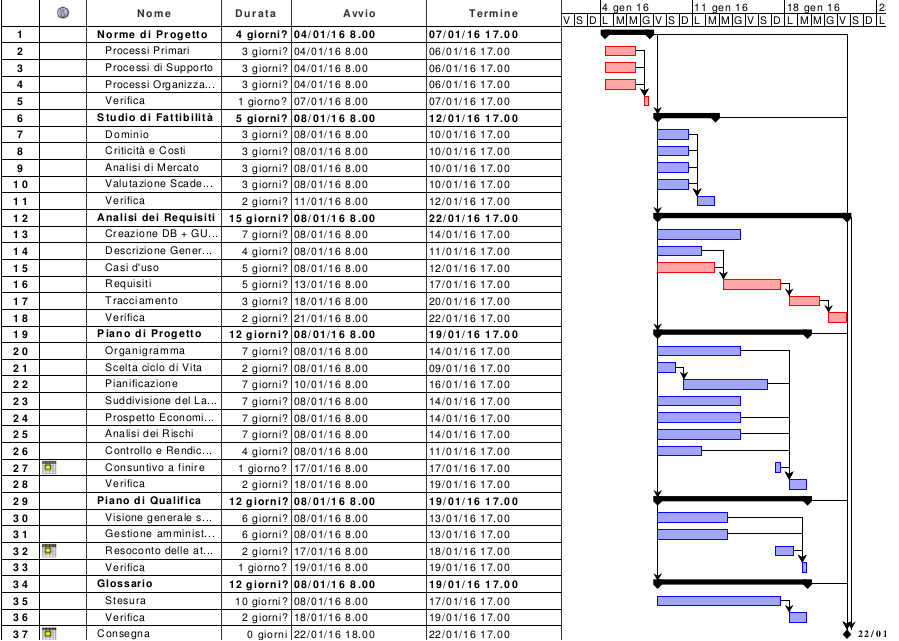
\includegraphics[width=\textwidth]{gantt_approccio}
					\caption{Diagramma di Gantt - fase di approccio al capitolato.}
				\end{figure}
			\subsubsection{WBS attività}
				%Image
				\begin{figure}[H]
					\centering
					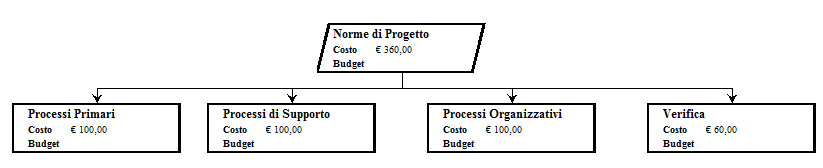
\includegraphics[width=\textwidth]{wbs/wbs_approccio_1}
					\caption{Work Breakdown Structure - fase di approccio al capitolato - norme di progetto. }
				\end{figure}
				\begin{figure}[H]
					\centering
					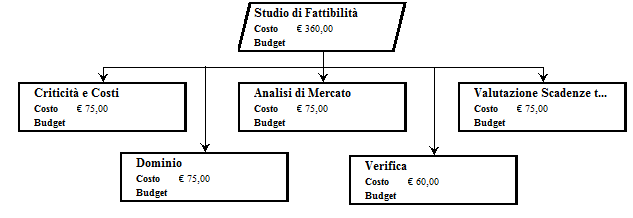
\includegraphics[width=\textwidth]{wbs/wbs_approccio_2}
					\caption{Work Breakdown Structure - fase di approccio al capitolato - studio di fattibilità.}
				\end{figure}
				\begin{figure}[H]
					\centering
					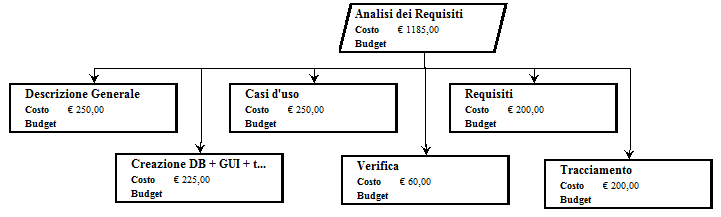
\includegraphics[width=\textwidth]{wbs/wbs_approccio_3}
					\caption{Work Breakdown Structure - fase di approccio al capitolato - amalisi dei requisiti}
				\end{figure}
				\begin{figure}[H]
					\centering
					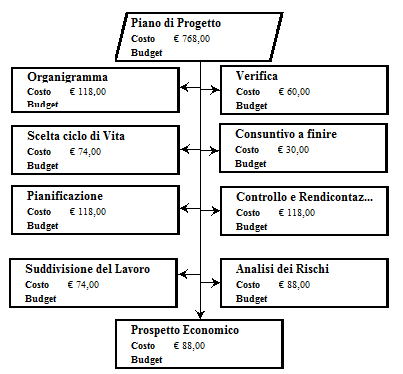
\includegraphics[width=\textwidth]{wbs/wbs_approccio_4}
					\caption{Work Breakdown Structure - fase di approccio al capitolato - piano di progetto.}
				\end{figure}
				\begin{figure}[H]
					\centering
					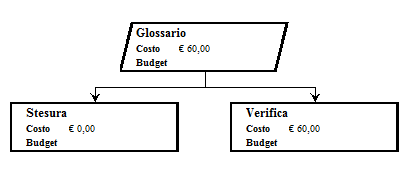
\includegraphics[width=\textwidth]{wbs/wbs_approccio_5}
					\caption{Work Breakdown Structure - fase di approccio al capitolato - glossario}
				\end{figure}
				\begin{figure}[H]
					\centering
					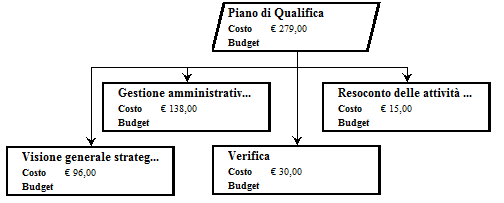
\includegraphics[width=\textwidth]{wbs/wbs_approccio_6}
					\caption{Work Breakdown Structure - fase di approccio al capitolato - piano di qualifica}
				\end{figure}
			\subsubsection{Ripartizione ore}
				%Image
				\begin{figure}[H]
					\centering
					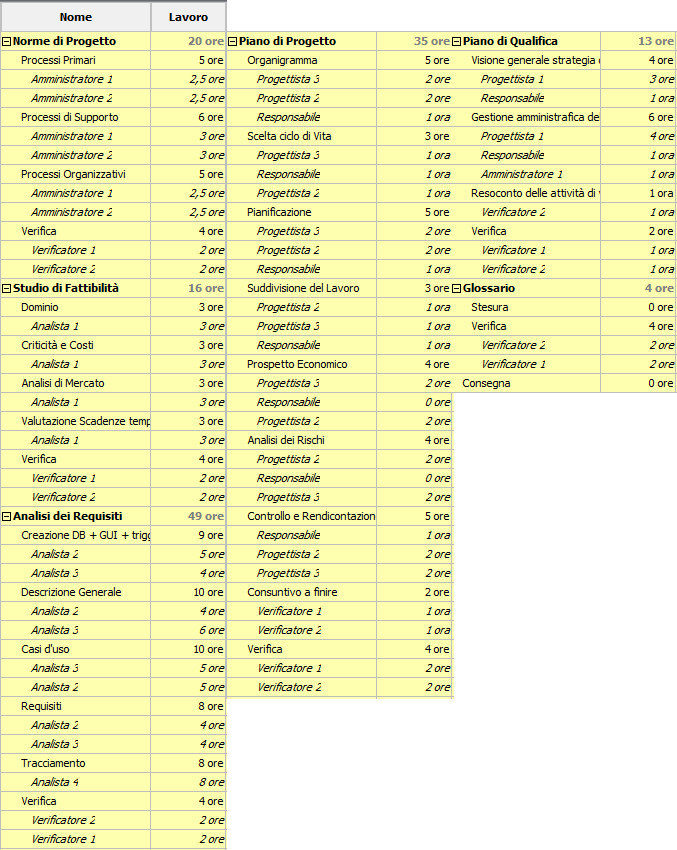
\includegraphics[width=\textwidth]{ro_approccio}
					\caption{Ripartizione ore - fase di approccio al capitolato.}
				\end{figure}

		\subsection{Analisi di dettaglio}
			\textbf{Periodo:} da 2016-01-23 a 2016-02-01 \\
			Questa fase inizio dopo la consegna dei documenti prevista per la \emph{Revisione dei requisiti}, corrispondente alla prima scadenza 
			che il gruppo intende rispettare e termina con l'inizio della fase successiva. In questa fase si migliorano i requisiti, suddividendo 
			quelli presenti in sotto-requisiti più specifici, viene aggiornato il documento di \emph{Analisi dei requisiti}.
			Le macro-attività sono le stesse della fase di \emph{Scelta ed approccio al capitolato}, escluso lo \emph{Studio di fattibilità}. 
			In questa fase i ruoli maggiormente coinvolti sono: \emph{Responsabile}, \emph{Amministratore} e \emph{Analista}.
			\subsubsection{Diagramma di Gantt}
				%Image
				\begin{figure}[H]
					\centering
					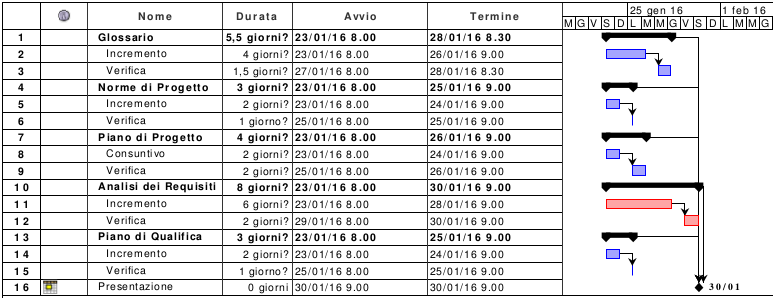
\includegraphics[width=\textwidth]{gantt_dettaglio}
					\caption{Diagramma di Gantt - fase di Analisi di dettaglio.}
				\end{figure}
			\subsubsection{WBS attività}
				%Image
				\begin{figure}[H]
					\centering
					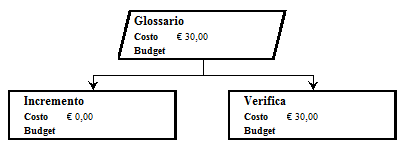
\includegraphics[width=\textwidth]{wbs/wbs_dettaglio_1}
					\caption{Work Breakdown Structure - fase di Analisi di dettaglio - glossario}
				\end{figure}
				\begin{figure}[H]
					\centering
					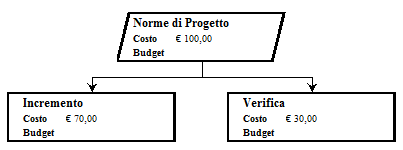
\includegraphics[width=\textwidth]{wbs/wbs_dettaglio_2}
					\caption{Work Breakdown Structure - fase di Analisi di dettaglio - norme di progetto}
				\end{figure}
				\begin{figure}[H]
					\centering
					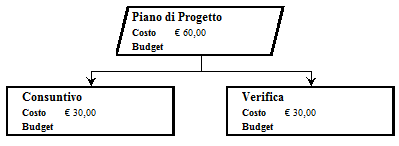
\includegraphics[width=\textwidth]{wbs/wbs_dettaglio_3}
					\caption{Work Breakdown Structure - fase di Analisi di dettaglio - piano di progetto}
				\end{figure}
				\begin{figure}[H]
					\centering
					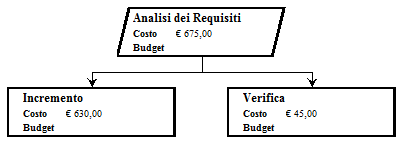
\includegraphics[width=\textwidth]{wbs/wbs_dettaglio_4}
					\caption{Work Breakdown Structure - fase di Analisi di dettaglio - analisi dei requisiti}
				\end{figure}
				\begin{figure}[H]
					\centering
					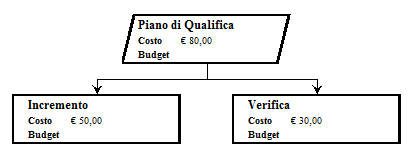
\includegraphics[width=\textwidth]{wbs/wbs_dettaglio_5}
					\caption{Work Breakdown Structure - fase di Analisi di dettaglio - piano di qualifica}
				\end{figure}
			\subsubsection{Ripartizione ore}
				%Image
				\begin{figure}[H]
					\centering
					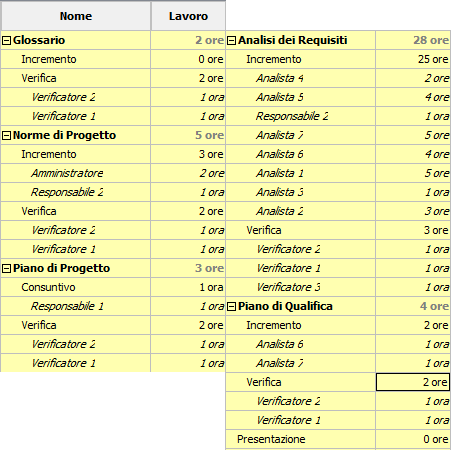
\includegraphics[width=\textwidth]{ro_dettaglio}
					\caption{Ripartizione ore - fase di esame dettagliato.}
				\end{figure}
				
		\subsection{Progettazione e sviluppo}
			\textbf{Periodo:} da 2016-02-01 a 2016-03-20 \\
			Questo periodo inizia al termine di quello di \emph{Analisi di dettaglio} e termina con la conclusione 
			della progettazione ad alto livello del progetto, prima della seconda scadenza. In questa fase viene 
			descritta la struttura logica ad alto livello del prodotto, mentre il suo stato definitivo viene 
			descritto nella fase successiva. \\
			Le macro-attività che saranno svolte durante questo periodo sono:
			\begin{itemize}
				\item \textbf{Specifica tecnica:} i progettisti del gruppo esporranno le scelte progettuali ad alto 
				livello che il prodotto dovrà assicurare. Verranno descritti i design pattern designati per lo sviluppo, 
				l'architettura generale del software, il tracciamento dei requisiti e i principali flussi di controllo;
				\item \textbf{Incremento e verifica:} tutti i documenti in questa macro-attività verranno aggiornati in base 
				al risultato della \emph{Revisione dei requisiti}.
			\end{itemize}
			In questo periodo i ruoli principalmente coinvolti sono: \emph{Responsabile}, \emph{Amministratore},
			\emph{Progettista}, \emph{Verificatore} e  \emph{Analista}.

			\subsubsection{Diagramma di Gantt}
				%Image
				\begin{figure}[H]
					\centering
					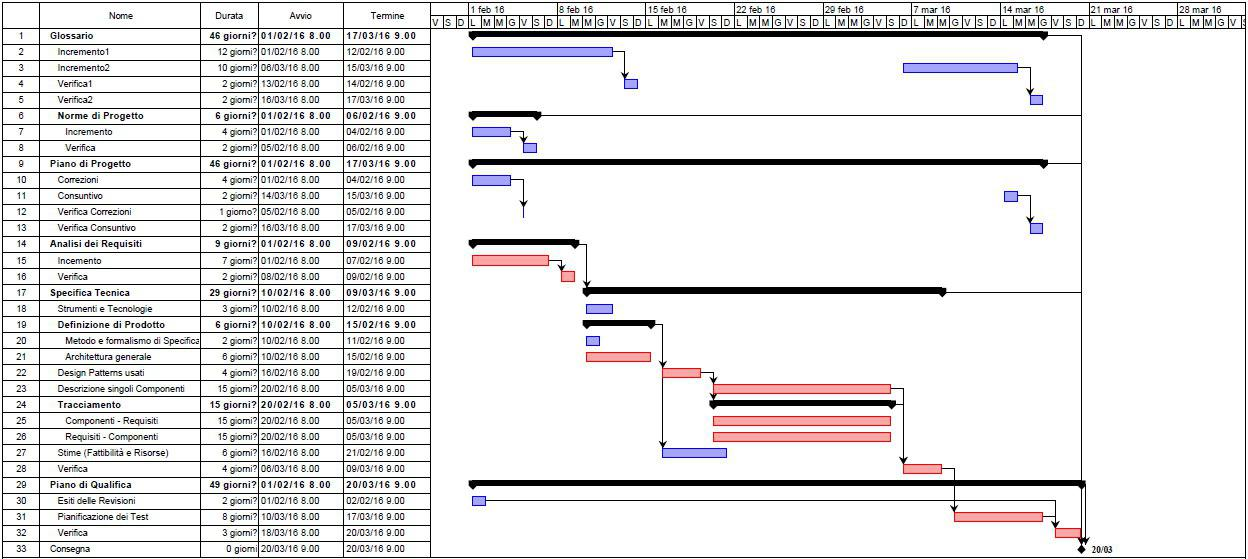
\includegraphics[width=\textwidth]{gantt_sviluppo}
					\caption{Diagramma di Gantt - fase di sviluppo.}
				\end{figure}
			\subsubsection{WBS attività}
				%Image
				\begin{figure}[H]
					\centering
					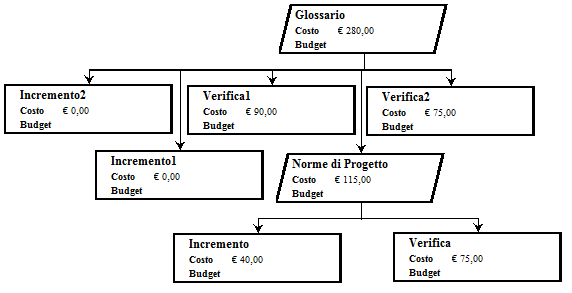
\includegraphics[width=\textwidth]{wbs/wbs_sviluppo_1}
					\caption{Work Breakdown Structure - fase di sviluppo - glossario}
				\end{figure}
				\begin{figure}[H]
					\centering
					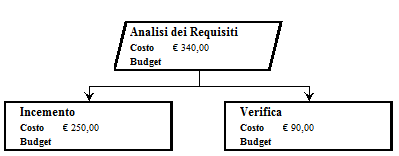
\includegraphics[width=\textwidth]{wbs/wbs_sviluppo_2}
					\caption{Work Breakdown Structure - fase di sviluppo - analisi dei requisiti}
				\end{figure}
				\begin{figure}[H]
					\centering
					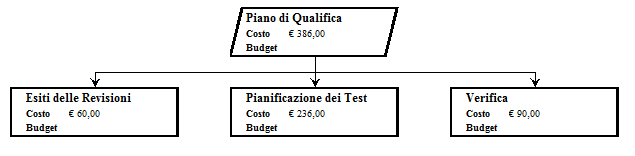
\includegraphics[width=\textwidth]{wbs/wbs_sviluppo_3}
					\caption{Work Breakdown Structure - fase di sviluppo - piano di qualifica}
				\end{figure}
				\begin{figure}[H]
					\centering
					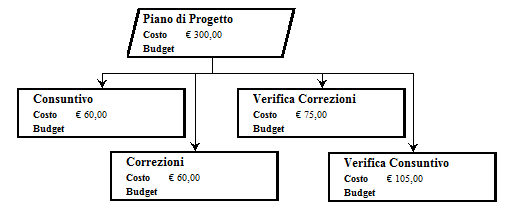
\includegraphics[width=\textwidth]{wbs/wbs_sviluppo_4}
					\caption{Work Breakdown Structure - fase di sviluppo - piano di progetto}
				\end{figure}
				\begin{figure}[H]
					\centering
					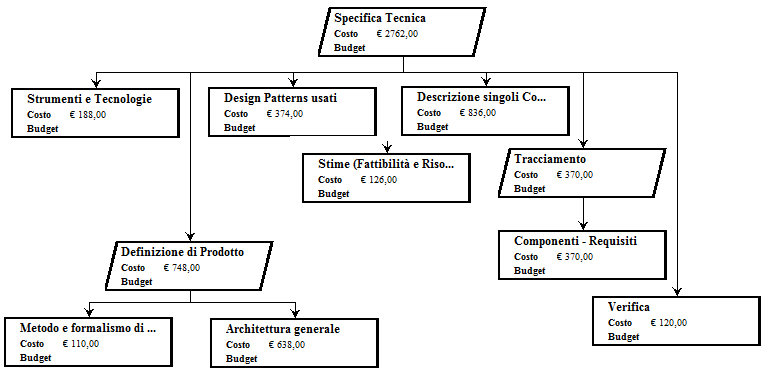
\includegraphics[width=\textwidth]{wbs/wbs_sviluppo_5}
					\caption{Work Breakdown Structure - fase di sviluppo - specifica tecnica}
				\end{figure}
			\subsubsection{Ripartizione ore}
				%Image
				\begin{figure}[H]
					\centering
					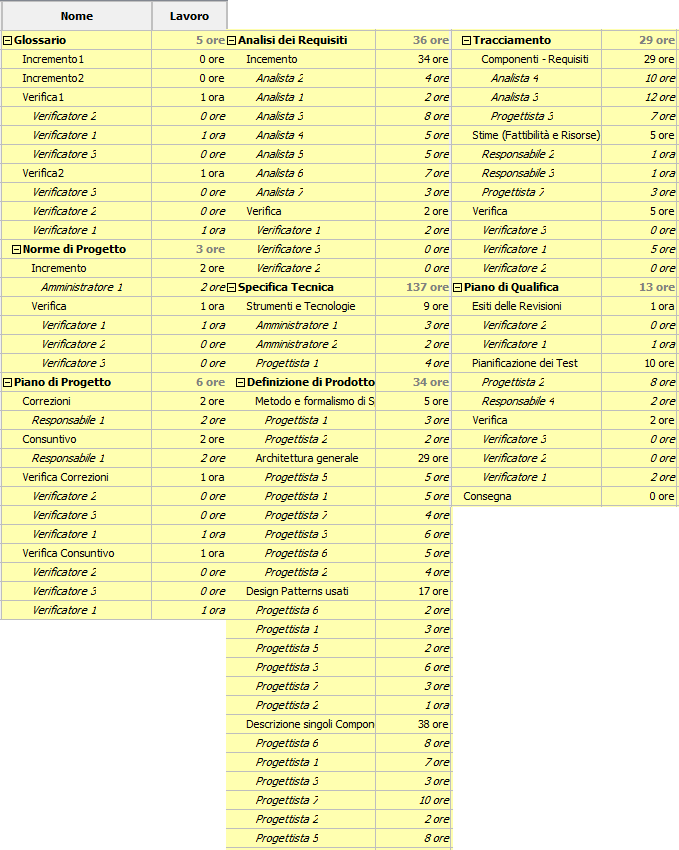
\includegraphics[width=\textwidth]{ro_sviluppo}
					\caption{Ripartizione ore - fase di sviluppo.}
				\end{figure}
				
		\subsection{Sviluppo ulteriore ed incremento}
			\textbf{Periodo:} da 2016-03-21 a 2016-05-23 \\
			
			Questa fase ha inizio immediatamente dopo la fine dello sviluppo, attraversa la seconda 
			scadenza che il gruppo intende rispettare, la \emph{Revisione di progetto} ed ha il compito di descrivere nel dettaglio 
			l'architettura del prodotto, e la sua realizzazione. La scadenza di questo periodo è definita dalla 
			\emph{Revisione di qualifica}. \\
			Le macro-attività principali di questo periodo sono:
			\begin{itemize}
				\item \textbf{Definizione di Prodotto:} in questa macro-attività viene definita in modo approfondito la struttura e le relazioni 
				dei vari componenti del prodotto, basandosi sul documento di \emph{Specifica tecnica}; 
				\item \textbf{Codifica:} Durante questa macro-attività ha inizio lo sviluppo del codice del prodotto da parte dei programmatori, 
				tenuti a seguire quanto specificato nel documento \emph{Definizione di prodotto};
				\item \textbf{Manuali utente:} questi documenti avranno lo scopo di illustrare delle linee guida per l'utilizzo 
				del sistema da parte degli utenti;
				\item \textbf{Incremento e verifica:} tutti i documenti verranno aggiornati per la presentazione alla 
				\emph{Revisione di qualifica}.
			\end{itemize}
			In questa fase i ruoli principalmente coinvolti sono: \emph{Responsabile}, \emph{Amministratore},
			\emph{Progettista} e \emph{Verificatore}.

			\subsubsection{Diagramma di Gantt}
				%Image
				\begin{figure}[H]
					\centering
					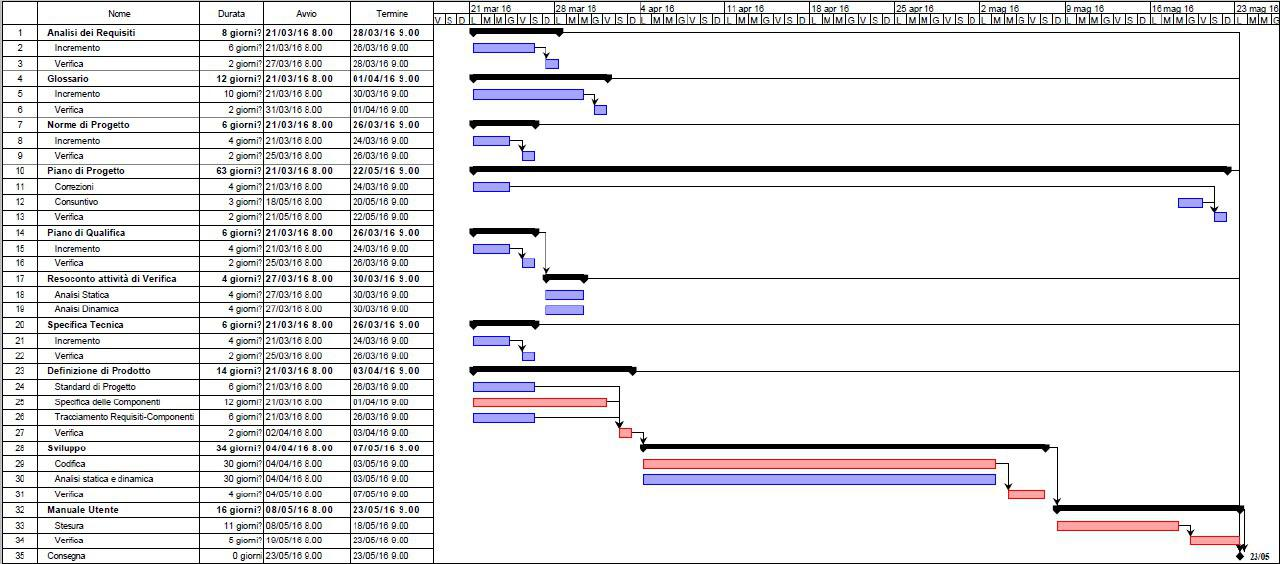
\includegraphics[width=\textwidth]{gantt_incremento}
					\caption{Diagramma di Gantt - fase di Incremento.}
				\end{figure}
			\subsubsection{WBS attività}
				%Image
				\begin{figure}[H]
					\centering
					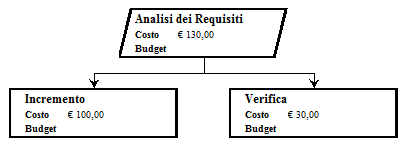
\includegraphics[width=\textwidth]{wbs/wbs_incremento_1}
					\caption{Work Breakdown Structure - fase di Incremento - analisi dei requisiti}
				\end{figure}
				\begin{figure}[H]
					\centering
					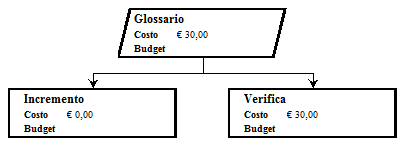
\includegraphics[width=\textwidth]{wbs/wbs_incremento_2}
					\caption{Work Breakdown Structure - fase di Incremento - glossario}
				\end{figure}
				\begin{figure}[H]
					\centering
					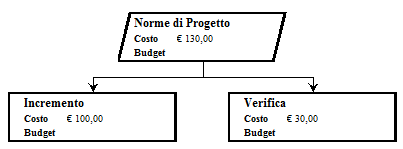
\includegraphics[width=\textwidth]{wbs/wbs_incremento_3}
					\caption{Work Breakdown Structure - fase di Incremento - norme di progetto}
				\end{figure}
				\begin{figure}[H]
					\centering
					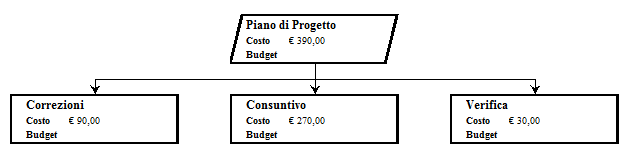
\includegraphics[width=\textwidth]{wbs/wbs_incremento_4}
					\caption{Work Breakdown Structure - fase di Incremento - piano di progetto}
				\end{figure}
				\begin{figure}[H]
					\centering
					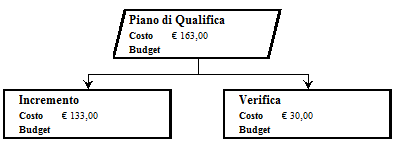
\includegraphics[width=\textwidth]{wbs/wbs_incremento_5}
					\caption{Work Breakdown Structure - fase di Incremento - piano di qualifica}
				\end{figure}
				\begin{figure}[H]
					\centering
					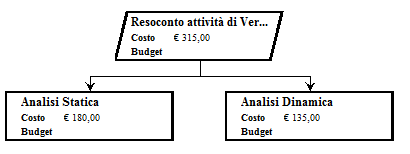
\includegraphics[width=\textwidth]{wbs/wbs_incremento_6}
					\caption{Work Breakdown Structure - fase di Incremento - resoconto}
				\end{figure}
				\begin{figure}[H]
					\centering
					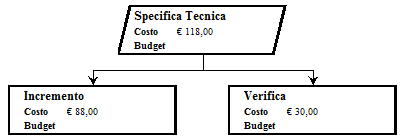
\includegraphics[width=\textwidth]{wbs/wbs_incremento_7}
					\caption{Work Breakdown Structure - fase di Incremento - specifica tecnica}
				\end{figure}
				\begin{figure}[H]
					\centering
					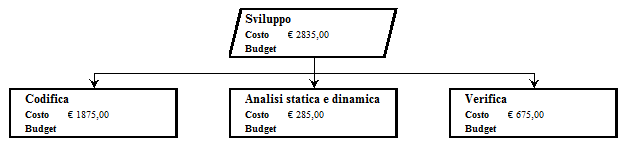
\includegraphics[width=\textwidth]{wbs/wbs_incremento_8}
					\caption{Work Breakdown Structure - fase di Incremento - sviluppo}
				\end{figure}
				\begin{figure}[H]
					\centering
					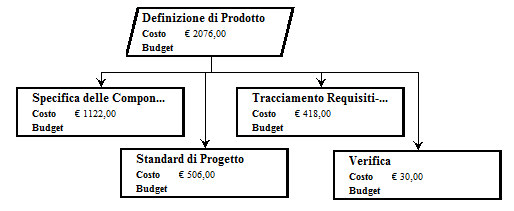
\includegraphics[width=\textwidth]{wbs/wbs_incremento_9}
					\caption{Work Breakdown Structure - fase di Incremento - definizione di prodotto}
				\end{figure}
				\begin{figure}[H]
					\centering
					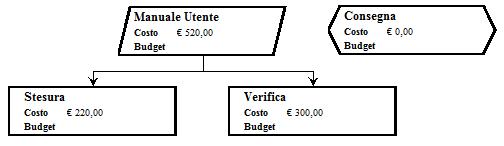
\includegraphics[width=\textwidth]{wbs/wbs_incremento_10}
					\caption{Work Breakdown Structure - fase di Incremento - manuale utente}
				\end{figure}
				
			\subsubsection{Ripartizione ore}
				%Image
				\begin{figure}[H]
					\centering
					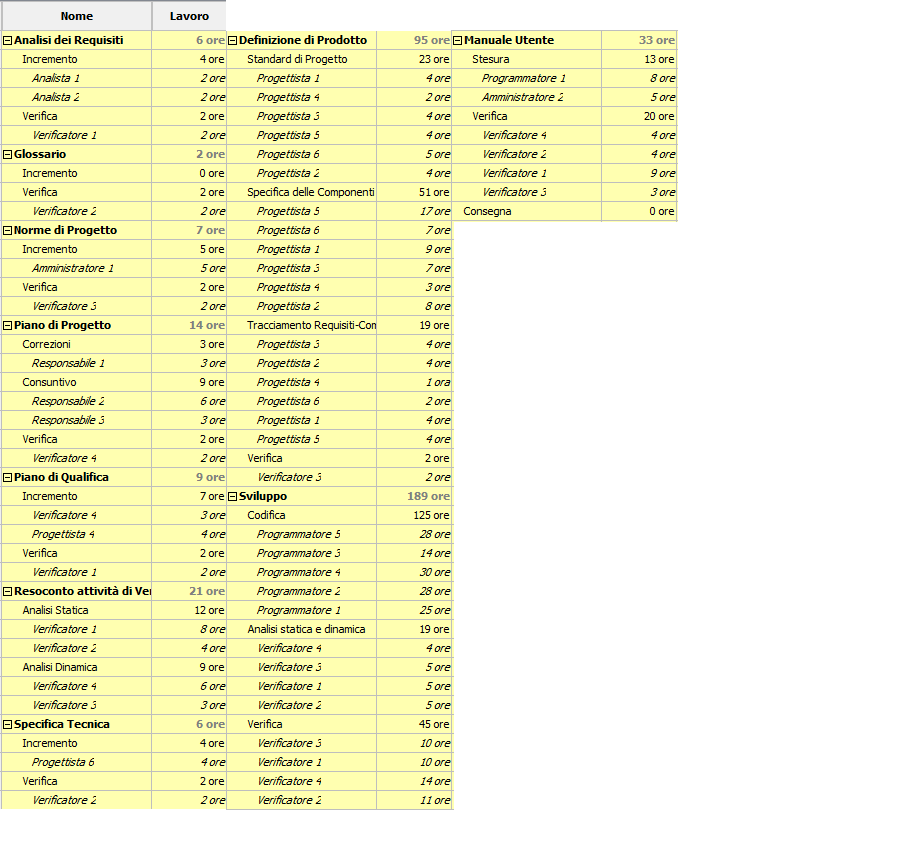
\includegraphics[width=\textwidth]{ro_incremento}
					\caption{Ripartizione ore - fase di Incremento.}
				\end{figure}
				
		\subsection{Conclusione}
			\textbf{Periodo:} da 2016-05-24 a 2016-06-19 \\
			
			Questa fase porta a compimento l'intero progetto, ed è successiva alla \emph{Revisione di qualifica}. In questa fase
			il gruppo intende effettuare gli ultimi test di verifica, di integrazione e la validazione del prodotto. 
			Questa fase termina la parte di ciclo di vita del software che il gruppo deve ricoprire, si chiude infatti nella data 
			dell'ultima consegna che il gruppo intende rispettare: \emph{Revisione di accettazione}.
			Durante questa fase sono include due principali macro-attività:
			\begin{itemize}
				\item \textbf{Ambiente di validazione e collaudo del sistema:} in questa macro-attività il prodotto verrà 
				convalidato, verrà quindi dimostrato che è conforme alle specifiche e soddisfa le richieste del committente;
				\item \textbf{Incremento e verifica:} tutti i documenti verranno aggiornati in base al risultato della 
				\emph{Revisione di qualifica} e preparati per la \emph{Revisione di accettazione}.
			\end{itemize}
			\subsubsection{Diagramma di Gantt}
				%Image
				\begin{figure}[H]
					\centering
					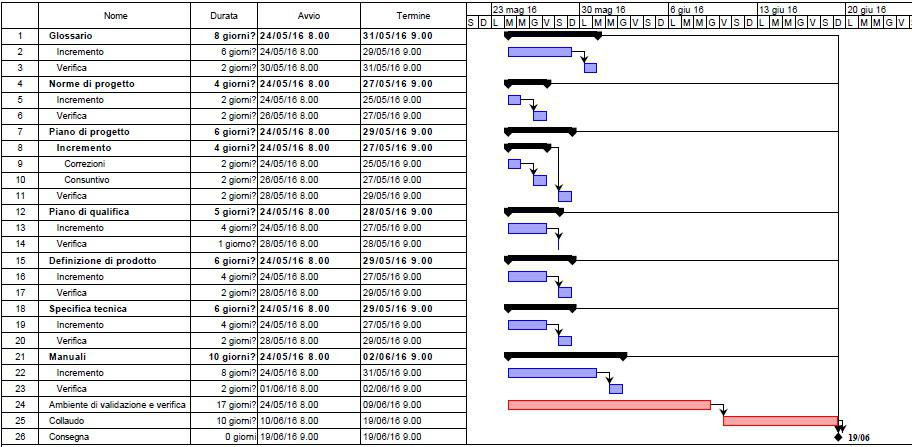
\includegraphics[width=\textwidth]{gantt_conclusione}
					\caption{Diagramma di Gantt - fase di Conclusione.}
				\end{figure}
			\subsubsection{WBS attività}
				%Image
				\begin{figure}[H]
					\centering
					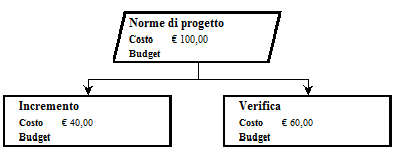
\includegraphics[width=\textwidth]{wbs/wbs_conclusione_1}
					\caption{Work Breakdown Structure - fase di Conclusione - norme di progetto}
				\end{figure}
				\begin{figure}[H]
					\centering
					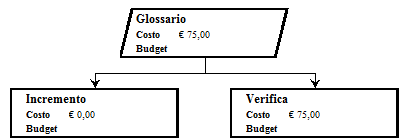
\includegraphics[width=\textwidth]{wbs/wbs_conclusione_2}
					\caption{Work Breakdown Structure - fase di Conclusione - glossario}
				\end{figure}
				\begin{figure}[H]
					\centering
					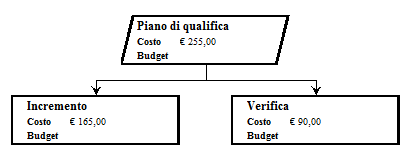
\includegraphics[width=\textwidth]{wbs/wbs_conclusione_3}
					\caption{Work Breakdown Structure - fase di Conclusione - piano di qualifica}
				\end{figure}
				\begin{figure}[H]
					\centering
					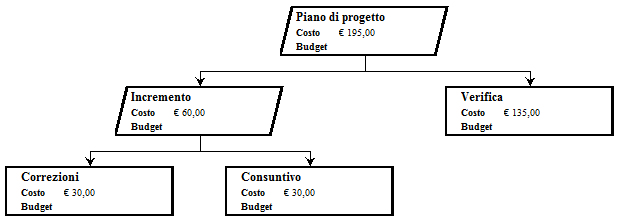
\includegraphics[width=\textwidth]{wbs/wbs_conclusione_4}
					\caption{Work Breakdown Structure - fase di Conclusione - piano di progetto}
				\end{figure}
				\begin{figure}[H]
					\centering
					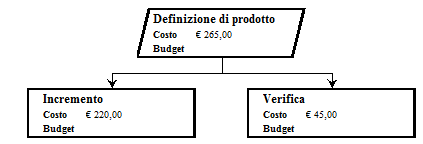
\includegraphics[width=\textwidth]{wbs/wbs_conclusione_5}
					\caption{Work Breakdown Structure - fase di Conclusione - definizione di prodotto}
				\end{figure}
				\begin{figure}[H]
					\centering
					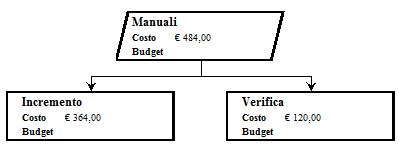
\includegraphics[width=\textwidth]{wbs/wbs_conclusione_6}
					\caption{Work Breakdown Structure - fase di Conclusione - manuali}
				\end{figure}
				\begin{figure}[H]
					\centering
					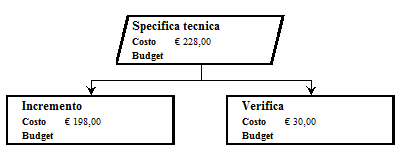
\includegraphics[width=\textwidth]{wbs/wbs_conclusione_8}
					\caption{Work Breakdown Structure - fase di Conclusione - specifica tecnica}
				\end{figure}
				\begin{figure}[H]
					\centering
					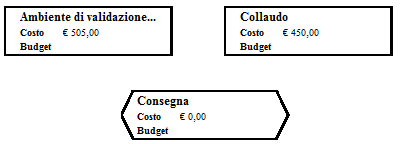
\includegraphics[width=\textwidth]{wbs/wbs_conclusione_7}
					\caption{Work Breakdown Structure - fase di Conclusione - validazione e collaudo}
				\end{figure}
			\subsubsection{Ripartizione ore}
				%Image
				\begin{figure}[H]
					\centering
					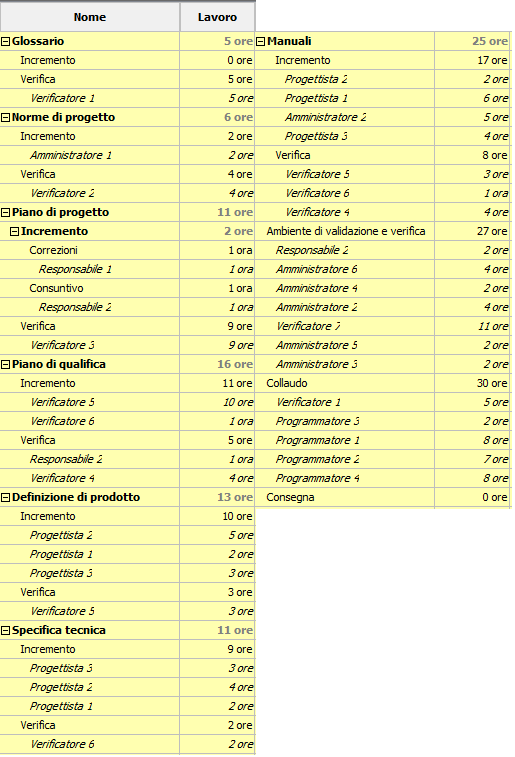
\includegraphics[width=\textwidth]{ro_conclusione}
					\caption{Ripartizione ore - fase di Conclusione.}
				\end{figure}

	\newpage 
	\section{Suddivisione del lavoro}
		Ogni membro del gruppo, dovrà, durante tutta la durata del progetto, ricoprire almeno una volta ciascuno dei
		ruoli descritti nell'appendice, sezione A.5. Durante ogni fase ogni membro può ricoprire
		più ruoli contemporaneamente, a patto che non si verifichino dei conflitti di interesse tra i ruoli ricoperti: 
		un membro del gruppo non può verificare il suo stesso lavoro.
		
		\subsection{Dettaglio delle fasi}

			\subsubsection{Scelta ed approccio al capitolato}
				Nella fase di \emph{Scelta ed approccio al capitolato} ciascun componente dovrà ricoprire i seguenti ruoli:
				\begin{table}[H]
					\begin{tabularx}{\textwidth}{ r t t t t t t | >{\centering\arraybackslash}t } 
						\rowcolor{orange!85}& \multicolumn{6}{c}{Ore per ruoli} &  \\
						\rowcolor{orange!85}Nominativo & Re & Am & An & Pt & Ve & Pr & Totali\\ 
						\noalign{\hrule height 1.5pt}
						\multicolumn{1}{r|}{Biggeri Mattia} & & & & 7 & 13 & & 20\\
						\multicolumn{1}{r|}{Bonato Paolo} & & & 18 & & & & 18\\ 
						\multicolumn{1}{r|}{Bortolazzo Matteo} & & & 19 & & & & 19\\ 
						\multicolumn{1}{r|}{Maino Elia} & & 8 & 12 & & & & 20\\
						\multicolumn{1}{r|}{Nicoletti Luca} & & 8 & & 12 & & & 20\\
						\multicolumn{1}{r|}{Padovan Tommaso} & 7 & & & 12 & & & 19\\
						\multicolumn{1}{r|}{Tommasin Davide} & & & 8 & & 12 & & 20\\
						\noalign{\hrule height 1.5pt}						
					\end{tabularx}
				\caption{Ripartizione ore - fase di Analisi. } 
				\label{TRAnalisi}
				\end{table}
				I valori sono rappresentati nel grafico, per semplificare la visualizzazione di quante ore ciascun membro 
				abbia dedicato ad un determinato ruolo.
				%Image
				\begin{figure}[H]
					\centering
					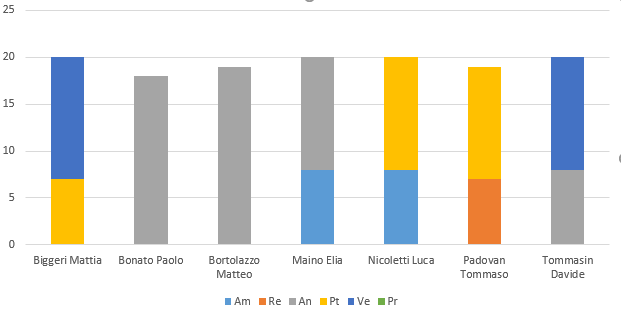
\includegraphics[scale=0.8]{bc_approccio.png}
					\caption{Ore per componente, fase di Analisi.}
				\end{figure}
				
			\subsubsection{Analisi di dettaglio}
				Nella fase di \emph{Analisi di dettaglio} ciascun componente dovrà ricoprire i seguenti ruoli:
				\begin{table}[H]
					\begin{tabularx}{\textwidth}{ r t t t t t t | >{\centering\arraybackslash}t } 
						\rowcolor{orange!85}& \multicolumn{6}{c}{Ore per ruoli} &  \\
						\rowcolor{orange!85}Nominativo & Re & Am & An & Pt & Ve & Pr & Totali\\ 
						\noalign{\hrule height 1.5pt}
						\multicolumn{1}{r|}{Biggeri Mattia} & & & 5 & & & & 5\\
						\multicolumn{1}{r|}{Bonato Paolo} & & 2 & 3 & & & & 5\\ 
						\multicolumn{1}{r|}{Bortolazzo Matteo} & & & 1 & & 5 & & 6\\ 
						\multicolumn{1}{r|}{Maino Elia} & & & 2 & & 5 & & 7\\
						\multicolumn{1}{r|}{Nicoletti Luca} & 2 & & 4 & & 1 & & 7\\
						\multicolumn{1}{r|}{Padovan Tommaso} & 1 & & 5 & & & & 6\\
						\multicolumn{1}{r|}{Tommasin Davide} & & & 6 & & & & 6\\
						\noalign{\hrule height 1.5pt}						
					\end{tabularx}
					\caption{Ripartizione ore - fase di Analisi di dettaglio. } 
					\label{TRDettaglio}
				\end{table}
				I valori sono rappresentati nel grafico, per semplificare la visualizzazione di quante ore ciascun membro 
				abbia dedicato ad un determinato ruolo.
				%Image
				\begin{figure}[H]
					\centering
					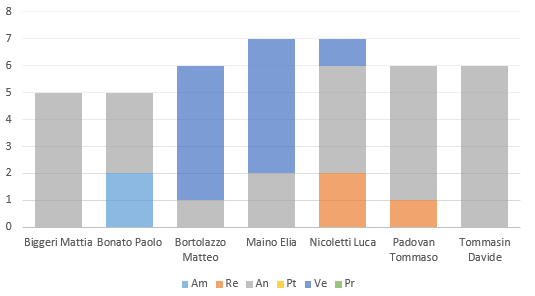
\includegraphics[scale=0.9]{bc_dettaglio.png}
					\caption{Ore per componente, fase di Analisi di dettaglio.}
				\end{figure}
				
			\subsubsection{Progettazione e sviluppo}
				Nella fase di \emph{Progettazione e sviluppo} ciascun componente dovrà ricoprire i seguenti ruoli:
				\begin{table}[H]
					\begin{tabularx}{\textwidth}{ r t t t t t t | >{\centering\arraybackslash}t } 
						\rowcolor{orange!85}& \multicolumn{6}{c}{Ore per ruoli} &  \\
						\rowcolor{orange!85}Nominativo & Re & Am & An & Pt & Ve & Pr & Totali\\ 
						\noalign{\hrule height 1.5pt}
						\multicolumn{1}{r|}{Biggeri Mattia} & 4 & & & 20 & & & 24\\
						\multicolumn{1}{r|}{Bonato Paolo} & & & 2 & 17 & 15 & & 34\\ 
						\multicolumn{1}{r|}{Bortolazzo Matteo} & 1 & & 4 & 22 & & & 27\\ 
						\multicolumn{1}{r|}{Maino Elia} & 1 & & & 5 & 22 & & 28\\
						\multicolumn{1}{r|}{Nicoletti Luca} & 2 & & & 15 & 15 & & 32\\
						\multicolumn{1}{r|}{Padovan Tommaso} & & 5 & 7 & 15 & & & 27\\
						\multicolumn{1}{r|}{Tommasin Davide} & & 2 & 3 & 20 & & & 25\\
						\noalign{\hrule height 1.5pt}						
					\end{tabularx}
					\caption{Ripartizione ore - fase di Progettazione e sviluppo. } 
					\label{TRProgettazione}
				\end{table}
				I valori sono rappresentati nel grafico, per semplificare la visualizzazione di quante ore ciascun membro 
				abbia dedicato ad un determinato ruolo.
				%Image
				\begin{figure}[H]
					\centering
					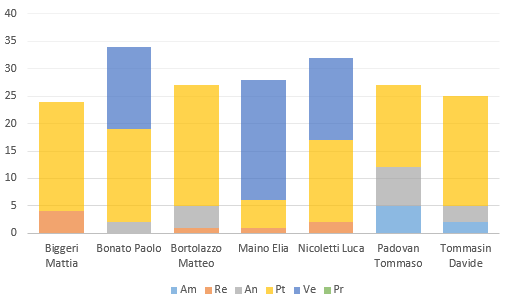
\includegraphics[scale=0.9]{bc_sviluppo.png}
					\caption{Ore per componente, fase di Progettazione e sviluppo.}
				\end{figure}
				
			\subsubsection{Sviluppo ulteriore ed incremento}
				Nella fase di \emph{Sviluppo ulteriore ed incremento} ciascun componente dovrà ricoprire i seguenti ruoli:
				\begin{table}[H]
					\begin{tabularx}{\textwidth}{ r t t t t t t | >{\centering\arraybackslash}t } 
						\rowcolor{orange!85}& \multicolumn{6}{c}{Ore per ruoli} &  \\
						\rowcolor{orange!85}Nominativo & Re & Am & An & Pt & Ve & Pr & Totali\\ 
						\noalign{\hrule height 1.5pt}
						\multicolumn{1}{r|}{Biggeri Mattia} & & 5 & & 17 & & 33 & 55\\
						\multicolumn{1}{r|}{Bonato Paolo} & 3 & & & 16 & 36 & & 55\\ 
						\multicolumn{1}{r|}{Bortolazzo Matteo} & 6 & 5 & & 15 & & 28 & 54\\ 
						\multicolumn{1}{r|}{Maino Elia} & 3 & & & 10 & 28 & 14 & 55\\
						\multicolumn{1}{r|}{Nicoletti Luca} & & & & 25 & & 30 & 55\\
						\multicolumn{1}{r|}{Padovan Tommaso} & & & 2 & & 25 & 28 & 55\\
						\multicolumn{1}{r|}{Tommasin Davide} & & & 2 & 18 & 33 & & 53\\
						\noalign{\hrule height 1.5pt}						
					\end{tabularx}
					\caption{Ripartizione ore - fase di Incremento.} 
					\label{TRCodifica}
				\end{table}
				I valori sono rappresentati nel grafico, per semplificare la visualizzazione di quante ore ciascun membro 
				abbia dedicato ad un determinato ruolo.
				%Image
				\begin{figure}[H]
					\centering
					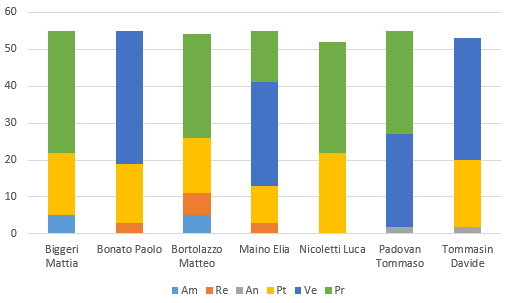
\includegraphics[scale=0.9]{bc_incremento.png}
					\caption{Ore per componente, fase di Incremento.}
				\end{figure}
				
			\subsubsection{Conclusione}
				Nella fase di \emph{Conclusione} ciascun componente dovrà ricoprire i seguenti ruoli:
				\begin{table}[H]
					\begin{tabularx}{\textwidth}{ r t t t t t t | >{\centering\arraybackslash}t } 
						\rowcolor{orange!85}& \multicolumn{6}{c}{Ore per ruoli} &  \\
						\rowcolor{orange!85}Nominativo & Re & Am & An & Pt & Ve & Pr & Totali\\ 
						\noalign{\hrule height 1.5pt}
						\multicolumn{1}{r|}{Biggeri Mattia} & & 2 & & & 10 & 8 & 20\\
						\multicolumn{1}{r|}{Bonato Paolo} & 1 & 9 & & & 4 & 7 & 21\\ 
						\multicolumn{1}{r|}{Bortolazzo Matteo} & & 2 & & 10 & 9 & & 21\\ 
						\multicolumn{1}{r|}{Maino Elia} & & 2 & & 11 & 8 & & 21\\
						\multicolumn{1}{r|}{Nicoletti Luca} & & & & 10 & 11 & & 21\\
						\multicolumn{1}{r|}{Padovan Tommaso} & & 2 & & & 16 & 2 & 20\\
						\multicolumn{1}{r|}{Tommasin Davide} & 4 & 4 & & & 4 & 8 & 20\\
						\noalign{\hrule height 1.5pt}						
					\end{tabularx}
					\caption{Ripartizione ore - fase di Conclusione. } 
					\label{TRVeV}
				\end{table}
				I valori sono rappresentati nel grafico, per semplificare la visualizzazione di quante ore ciascun membro 
				abbia dedicato ad un determinato ruolo.
				%Image
				\begin{figure}[H]
					\centering
					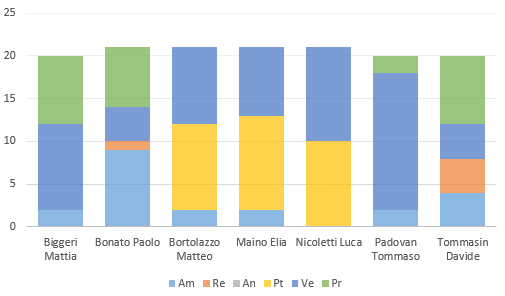
\includegraphics[scale=0.9]{bc_conclusione.png}
					\caption{Ore per componente, fase di Conclusione.}
				\end{figure}
				
		\subsection{Totali}
			\subsubsection{Totale ore}
				Nel calcolo totale delle ore che il gruppo intende dedicare allo svolgimento del progetto, vengono inserite anche le ore
				di investimento, appartenenti al periodo di \emph{Approccio al capitolato}, che vengono invece omesse dal calcolo del 
				preventivo. Le ore che ciascun membro dedicherà al progetto saranno le seguenti:
				\begin{table}[H]
					\begin{tabularx}{\textwidth}{ r t t t t t t | >{\centering\arraybackslash}t } 
						\rowcolor{orange!85}& \multicolumn{6}{c}{Ore per ruoli} &  \\
						\rowcolor{orange!85}Nominativo & Re & Am & An & Pt & Ve & Pr & Totali\\ 
						\noalign{\hrule height 1.5pt}
						\multicolumn{1}{r|}{Biggeri Mattia} & 4 & 7 & 5 & 44 & 23 & 41 & 124\\
						\multicolumn{1}{r|}{Bonato Paolo} & 4 & 11 & 23 & 33 & 55 & 7 & 133\\ 
						\multicolumn{1}{r|}{Bortolazzo Matteo} & 7 & 7 & 24 & 47 & 14 & 28 & 127\\ 
						\multicolumn{1}{r|}{Maino Elia} & 4 & 10 & 14 & 26 & 63 & 14 & 131\\
						\multicolumn{1}{r|}{Nicoletti Luca} & 4 & 8 & 4 & 62 & 27 & 30 & 135\\
						\multicolumn{1}{r|}{Padovan Tommaso} & 8 & 7 & 14 & 27 & 41 & 30 & 127\\
						\multicolumn{1}{r|}{Tommasin Davide} & 4 & 6 & 19 & 38 & 49 & 8 & 124\\
						\noalign{\hrule height 1.5pt}						
					\end{tabularx}
					\caption{Ripartizione ore - totale ore. } 
					\label{TRTotale}
				\end{table}
				I valori sono rappresentati nel grafico, per semplificare la visualizzazione di quante ore ciascun membro 
				abbia dedicato ad un determinato ruolo.
				%Image
				\begin{figure}[H]
					\centering
					\includegraphics[scale=0.9]{bc_totali.png}
					\caption{Ore per componente, fase di Verifica e validazione.}
				\end{figure}
			\subsubsection{Totale ore rendicontate}
				Le ore espresse qui sotto, ovvero le ore che sono incluse nel calcolo del preventivo, sono minori rispetto a quelle 
				totali, in quanto non sono messe a carico del committente le ore appartenenti al periodo di \emph{Scelta ed approccio al capitolato}: 
				considerate come ore di investimento; inoltre, per evitare di superare il monte ore previsto, alcune ore sono state rimosse da quelle 
				rendicontate e spostate tra quelle di investimento in quanto esse superavano il limite massimo imposto dal progetto didattico. 
				\begin{table}[H]
					\begin{tabularx}{\textwidth}{ r t t t t t t | >{\centering\arraybackslash}t } 
						\rowcolor{orange!85}& \multicolumn{6}{c}{Ore per ruoli} &  \\
						\rowcolor{orange!85}Nominativo & Re & Am & An & Pt & Ve & Pr & Totali\\ 
						\noalign{\hrule height 1.5pt}
						\multicolumn{1}{r|}{Biggeri Mattia} & 4 & 7 & & 37 & 10 & 41 & 99\\
						\multicolumn{1}{r|}{Bonato Paolo} & 4 & 9 & 2 & 28 & 55 & 7 & 105\\ 
						\multicolumn{1}{r|}{Bortolazzo Matteo} & 7 & 7 & 4 & 47 & 9 & 28 & 102\\ 
						\multicolumn{1}{r|}{Maino Elia} & 4 & 2 & & 26 & 58 & 14 & 104\\
						\multicolumn{1}{r|}{Nicoletti Luca} & 2 & & & 50 & 23 & 30 & 105\\
						\multicolumn{1}{r|}{Padovan Tommaso} & & 7 & 9 & 15 & 41 & 30 & 102\\
						\multicolumn{1}{r|}{Tommasin Davide} & 4 & 6 & 5 & 38 & 37 & 8 & 98\\
						\noalign{\hrule height 1.5pt}						
					\end{tabularx}
					\caption{Ripartizione ore - totale rendicontate. } 
					\label{TRRendicontate}
				\end{table}
				I valori sono rappresentati nel grafico, per semplificare la visualizzazione di quante ore ciascun membro 
				abbia dedicato ad un determinato ruolo.
				%Image
				\begin{figure}[H]
					\centering
					\includegraphics[scale=0.9]{bc_rendicontate.png}
					\caption{Ore per componente, totale in preventivo.}
				\end{figure}
				
	\newpage 
	\section{Prospetto economico}
	
		Per ciascuna fase del progetto, in questa sezione vengono presentate le ore di impiego per tutti i 
		ruoli coinvolti. Si ricorda che le fasi di \emph{Scelta ed approccio al capitolato} e \emph{Analisi di dettaglio} non sono 
		a carico del committente e quindi non saranno considerate nel calcolo delle ore in preventivo.
		
		\subsection{Scelta ed approccio al capitolato}
			Nelle fase di \emph{Scelta ed approccio al capitolato}, le ore per ciascun ruolo sono state suddivise in questo modo:
			\begin{table}[H]
				\begin{tabularx}{\textwidth}{Y Y Y}
					\noalign{\hrule height 1.5pt}
					\rowcolor{orange!85}Ruolo & Ore & Costo \\
					\noalign{\hrule height 1.5pt}
					Responsabile & 7 & 210 \\
					Amministratore & 16 & 320 \\
					Analista & 57 & 1425\\
					Progettista & 31 & 682\\
					Verificatore & 25 & 375\\
					Programmatore & 0 & 0 \\
					\noalign{\hrule height 0.5pt}
					\textbf{Totali} & 136 & 3012 \\
					\noalign{\hrule height 1.5pt}
				\end{tabularx}
				\caption{Costo ore - fase di Scelta ed approccio al capitolato. } 
				\label{TCAnalisi}
			\end{table}
			I seguenti grafici mostrano come ogni ruolo e il rispettivo costo abbiano influito sul calcolo del totale 
			costo della fase di \emph{Scelta ed approccio al capitolato}.
			%Image
			\begin{figure}[H]
				\centering
				\includegraphics[scale=0.7]{pc_approccio}
				\caption{Ore per ruolo, fase di Scelta ed approccio al capitolato.}
			\end{figure}
			%Image
			\begin{figure}[H]
				\centering
				\includegraphics[scale=0.7]{pc_costi_approccio}
				\caption{Costi per ruolo, fase di Scelta ed approccio al capitolato.}
			\end{figure}
			
		\subsection{Analisi di dettaglio}
			Nelle fase di \emph{Analisi di dettaglio}, le ore per ciascun ruolo sono state suddivise in questo modo:
			\begin{table}[H]
				\begin{tabularx}{\textwidth}{Y Y Y}
					\noalign{\hrule height 1.5pt}
					\rowcolor{orange!85}Ruolo & Ore & Costo \\
					\noalign{\hrule height 1.5pt}
					Responsabile & 3 & 90 \\
					Amministratore & 2 & 40 \\
					Analista & 26 & 650\\
					Progettista & 0 & 0\\
					Verificatore & 11 & 165\\
					Programmatore & 0 & 0 \\
					\noalign{\hrule height 0.5pt}
					\textbf{Totali} & 42 & 945 \\
					\noalign{\hrule height 1.5pt}
				\end{tabularx}
				\caption{Costo ore - fase di Analisi di dettaglio. } 
				\label{TCDettaglio}
			\end{table}
			I seguenti grafici mostrano come ogni ruolo e il rispettivo costo abbiano influito sul calcolo del totale 
			costo della fase di \emph{Analisi di dettaglio}.
			%Image
			\begin{figure}[H]
				\centering
				\includegraphics[scale=0.7]{pc_dettaglio}
				\caption{Ore per ruolo, fase di Analisi di dettaglio.}
			\end{figure}
			%Image
			\begin{figure}[H]
				\centering
				\includegraphics[scale=0.7]{pc_costi_dettaglio}
				\caption{Costi per ruolo, fase di Analisi di dettaglio.}
			\end{figure}
			
		\subsection{Progettazione e sviluppo}
			Nelle fase di \emph{Progettazione e sviluppo}, le ore per ciascun ruolo sono state suddivise in questo modo:
			\begin{table}[H]
				\begin{tabularx}{\textwidth}{Y Y Y}
					\noalign{\hrule height 1.5pt}
					\rowcolor{orange!85}Ruolo & Ore & Costo \\
					\noalign{\hrule height 1.5pt}
					Responsabile & 8 & 240 \\
					Amministratore & 7 & 140 \\
					Analista & 16 & 400\\
					Progettista & 114 & 2508\\
					Verificatore & 52 & 780\\
					Programmatore & 0 & 0 \\
					\noalign{\hrule height 0.5pt}
					\textbf{Totali} & 197 & 4068 \\
					\noalign{\hrule height 1.5pt}
				\end{tabularx}
				\caption{Costo ore - fase di Progettazione e sviluppo. } 
				\label{TCProgettazione}
			\end{table}
			I seguenti grafici mostrano come ogni ruolo e il rispettivo costo abbiano influito sul calcolo del totale 
			costo della fase di \emph{Progettazione architetturale}.
			%Image
			\begin{figure}[H]
				\centering
				\includegraphics[scale=0.7]{pc_sviluppo}
				\caption{Ore per ruolo, fase di Progettazione e sviluppo.}
			\end{figure}
			%Image
			\begin{figure}[H]
				\centering
				\includegraphics[scale=0.7]{pc_costi_sviluppo}
				\caption{Costi per ruolo, fase di Progettazione e sviluppo.}
			\end{figure}
			
		\subsection{Sviluppo ulteriore ed incremento}
			Nelle fase di \emph{Sviluppo ulteriore ed incremento} le ore per ciascun ruolo sono state suddivise in questo modo:
			\begin{table}[H]
				\begin{tabularx}{\textwidth}{Y Y Y}
					\noalign{\hrule height 1.5pt}
					\rowcolor{orange!85}Ruolo & Ore & Costo \\
					\noalign{\hrule height 1.5pt}
					Responsabile & 12 & 360 \\
					Amministratore & 10 & 200 \\
					Analista & 4 & 100\\
					Progettista & 101 & 2222\\
					Verificatore & 122 & 1830\\
					Programmatore & 133 & 1995 \\
					\noalign{\hrule height 0.5pt}
					\textbf{Totali} & 382 & 6707 \\
					\noalign{\hrule height 1.5pt}
				\end{tabularx}
				\caption{Costo ore - fase di Sviluppo ulteriore ed incremento. }
				\label{TCCodifica}
			\end{table}
			I seguenti grafici mostrano come ogni ruolo e il rispettivo costo abbiano influito sul calcolo del totale 
			costo della fase di \emph{Progettazione di dettaglio e codifica}.
			%Image
			\begin{figure}[H]
				\centering
				\includegraphics[scale=0.7]{pc_incremento}
				\caption{Ore per ruolo, fase di Sviluppo ulteriore ed incremento.}
			\end{figure}
			%Image
			\begin{figure}[H]
				\centering
				\includegraphics[scale=0.7]{pc_costi_incremento}
				\caption{Costi per ruolo, fase di Sviluppo ulteriore ed incremento.}
			\end{figure}
			
		\subsection{Conclusione}
			Nelle fase di \emph{Conclusione}, le ore per ciascun ruolo sono state suddivise in questo modo:
			\begin{table}[H]
				\begin{tabularx}{\textwidth}{Y Y Y}
					\noalign{\hrule height 1.5pt}
					\rowcolor{orange!85}Ruolo & Ore & Costo \\
					\noalign{\hrule height 1.5pt}
					Responsabile & 5 & 150 \\
					Amministratore & 21 & 420 \\
					Analista & 0 & 0\\
					Progettista & 31 & 682\\
					Verificatore & 62 & 930\\
					Programmatore & 25 & 375 \\
					\noalign{\hrule height 0.5pt}
					\textbf{Totali} & 144 & 2557 \\
					\noalign{\hrule height 1.5pt}
				\end{tabularx}
				\caption{Costo ore - fase di Conclusione. } 
				\label{TCVeV}
			\end{table}
			I seguenti grafici mostrano come ogni ruolo e il rispettivo costo abbiano influito sul calcolo del totale 
			costo della fase di \emph{Conclusione}.
			%Image
			\begin{figure}[H]
				\centering
				\includegraphics[scale=0.7]{pc_conclusione}
				\caption{Ore per ruolo, fase di Conclusione.}
			\end{figure}
			%Image
			\begin{figure}[H]
				\centering
				\includegraphics[scale=0.7]{pc_costi_conclusione}
				\caption{Costi per ruolo, fase di Conclusione.}
			\end{figure}
			
		\subsection{Totali}
		
			Di seguito vengono riportate le somme delle ore impiegate durante tutte le fasi per lo svolgimento del progetto.
			Le ore nella sezione di \hyperref[SezTotaliInvestimento]{Investimento} comprendono le ore a carico del committente e le 
			ore di investimento, escluse invece dal preventivo in quanto a carico del gruppo. 
			
			\subsubsection{Investimento}
			\label{SezTotaliInvestimento}
				Le ore totali previste per la realizzazione del progetto sono riportate nella tabella seguente:
				
				\begin{table}[H]
					\begin{tabularx}{\textwidth}{Y Y Y}
						\noalign{\hrule height 1.5pt}
						\rowcolor{orange!85}Ruolo & Ore & Costo \\
						\noalign{\hrule height 1.5pt}
						Responsabile & 35 & 1050 \\
						Amministratore & 56 & 1120 \\
						Analista & 103 & 2575\\
						Progettista & 277 & 6094\\
						Verificatore & 272 & 4080\\
						Programmatore & 158 & 2370 \\
						\noalign{\hrule height 0.5pt}
						\textbf{Totali} & 901 & 17289 \\
						\noalign{\hrule height 1.5pt}
					\end{tabularx}
				\caption{Costo ore - totale con investimento. } 
				\label{TCTotaleInvestimento}
				\end{table}
				
				I seguenti grafici mostrano come ogni ruolo e il rispettivo costo abbiano influito sul calcolo del totale 
				costo della realizzazione del progetto.
				%Image
				\begin{figure}[H]
					\centering
					\includegraphics[scale=0.7]{pc_totali}
					\caption{Ore per ruolo, intero progetto.}
				\end{figure}
				%Image
				\begin{figure}[H]
					\centering
					\includegraphics[scale=0.7]{pc_costi_totali}
					\caption{Costi per ruolo, intero progetto.}
				\end{figure}
				
			\subsubsection{Preventivo}
				Le ore totali previste per la realizzazione del progetto e a carico del committente sono riportate 
				nella seguente tabella:
				\begin{table}[H]
					\begin{tabularx}{\textwidth}{Y Y Y}
						\noalign{\hrule height 1.5pt}
						\rowcolor{orange!85}Ruolo & Ore & Costo \\
						\noalign{\hrule height 1.5pt}
						Responsabile & 25 & 750 \\
						Amministratore & 38 & 760 \\
						Analista & 20 & 500\\
						Progettista & 246 & 5412\\
						Verificatore & 236 & 3540\\
						Programmatore & 158 & 2370 \\
						\noalign{\hrule height 0.5pt}
						\textbf{Totali} & 723 & 13332 \\
						\noalign{\hrule height 1.5pt}
					\end{tabularx}
				\caption{Costo ore - totale rendicontate.}
				\label{TCRendicontati}
				\end{table}
				I seguenti grafici mostrano come ogni ruolo e il rispettivo costo abbiano influito sul calcolo del totale 
				costo a carico del committente
				%Image
				\begin{figure}[H]
					\centering
					\includegraphics[scale=0.7]{pc_rendicontate}
					\caption{Ore per ruolo, rendicontate.}
				\end{figure}
				%Image
				\begin{figure}[H]
					\centering
					\includegraphics[scale=0.7]{pc_costi_rendicontate}
					\caption{Costi per ruolo, rendicontati.}
				\end{figure}
				
			\subsubsection{Conclusione}
				Il costo totale per lo sviluppo del progetto, indicato nella \hyperref[TCRendicontati]{Tabella 4.19} viene 
				arrotondato a 13.500\euro. L'arrotondamento per eccesso è una precauzione in quanto le stime di ore di lavoro 
				necessarie per ogni task e attività potrebbero rilevarsi insufficienti. In questo modo, anche sforando di qualche 
				ora il gruppo è assicurato, e riuscirà più facilmente a rimanere all'interno dei costi preventivati.
				
				Inoltre, se uno dei rischi successivamente analizzati dovesse presentarsi, il gruppo avrà comunque a disposizione 
				un monte ore non nullo per rimediare ai danni causati dal verificarsi del rischio.

	\newpage 
	\section{Consuntivo}
	\label{Consuntivo}
	
		Questa sezione, lasciata per ultima perché incrementale, riporta il prospetto economico con i 
		costi effettivamente sostenuti. Per ogni fase verrà calcolato un conguaglio, ovvero la differenza
		tra ore preventivate e spese, esso potrà essere:
		\begin{itemize}
			\item \textbf{Positivo:} se il preventivo ha superato il consuntivo;
			\item \textbf{In pari:} se il preventivo e il consuntivo coincidono;
			\item \textbf{Negativo:} se il consuntivo ha superato il preventivo.
		\end{itemize}
		
		\subsection{Scelta ed approccio al capitolato}
			Si riporta di seguito il consuntivo di periodo della fase di \emph{Scelta ed approccio al capitolato}. \\
			La tabella sottostante riporta le differenze delle ore tra preventivo e consuntivo, divise per ruolo. 
			Un segno positivo indica che sono state necessarie più ore del previsto, un segno negativo indica che sono 
			state impiegate meno ore di quelle presenti nel preventivo.
						
			\begin{table}[H]
				\begin{tabularx}{\textwidth}{Y Y Y}
					\noalign{\hrule height 1.5pt}
					\rowcolor{orange!85}Ruolo & Ore & Costo \\
					\noalign{\hrule height 1.5pt}
					Responsabile & -\space 1 & -\space 30 \\
					Amministratore & 0 & 0 \\
					Analista & -\space 2 & -\space 50\\
					Progettista & +\space 1 & +\space 22\\
					Verificatore & +\space 2 & +\space 20\\
					Programmatore & 0 & 0 \\
					\noalign{\hrule height 0.5pt}
					\textbf{Totali} & 0 & -\space 38 \\
					\noalign{\hrule height 1.5pt}
				\end{tabularx}
				\caption{Differenza consuntivo/preventivo - fase di Scelta ed approccio al capitolato. } 
				\label{ConsuntivoApproccio}
			\end{table}
			\subsubsection{Conclusioni}
				Lo svolgimento della fase di \emph{Scelta ed approccio al capitolato} discosta leggermente da quello programmato e 
				visualizzabile nel \emph{Gantt}. Il gruppo ha impiegato lo stesso monte ore previste, ma 
				ricoprendo ruoli diversi da quelli previsti, portando ad un conguaglio positivo.
				
				Tale differenza non influenzerà in alcun modo il costo totale del progetto in quanto le ore 
				di lavoro in questa fase non sono a carico del committente e vengono quindi omesse dal preventivo.
				
		\subsection{Analisi di dettaglio}
			Si riporta di seguito, come per la fase precedente, il consuntivo di periodo riguardante la fase di \emph{Analisi di dettaglio}. \\
			La tabella sottostante riporta le differenze delle ore tra preventivo e consuntivo, divise per ruolo.
			Il significato di segni positivi e negativi è lo stesso che nella \hyperref[DCSceltaCapitolato]{Tabella 20}.
			
			\begin{table}[H]
				\begin{tabularx}{\textwidth}{Y Y Y}
					\noalign{\hrule height 1.5pt}
					\rowcolor{orange!85}Ruolo & Ore & Costo \\
					\noalign{\hrule height 1.5pt}
					Responsabile & 0 & 0 \\
					Amministratore & 0 & 0 \\
					Analista & 0 & 0\\
					Progettista & 0 & 0\\
					Verificatore & 0 & 0\\
					Programmatore & 0 & 0 \\
					\noalign{\hrule height 0.5pt}
					\textbf{Totali} & 0 & 0 \\
					\noalign{\hrule height 1.5pt}
				\end{tabularx}
				\caption{Differenza consuntivo/preventivo - fase di Analisi di dettaglio. } 
				\label{ConsuntivoDettaglio}
			\end{table}
			
			\subsubsection{Conclusioni}
				Lo svolgimento di questa fase, essendo stata programmata in piccolo (ha infatti una durata di soli 9 giorni) è stato
				completamente rispettato in quanto ogni membro del gruppo ha rispettato le ore programmate. Il conguaglio è in pari e non 
				vi sono variazioni nel preventivo, anche perché le ore spese durante questa fase rientrano tra quelle da considerarsi di 
				investimento, e quindi non a carico del committente. 
			
		
			\subsection{Progettazione e sviluppo}
                Si riporta di seguito il consuntivo di periodo della fase di \emph{Progettazione e sviluppo}. \\
                La tabella sottostante riporta la differenza di ore tra preventivo e consuntivo, divise per ruolo. Il significato dei segni
                positivi e negativi è lo stesso che nella \hyperref[DCSceltaCapitolato]{Tabella 20}.
                \begin{table}[H]
					\begin{tabularx}{\textwidth}{Y Y Y}
						\noalign{\hrule height 1.5pt}
						\rowcolor{orange!85}Ruolo & Ore & Costo \\
						\noalign{\hrule height 1.5pt}
						Responsabile & -\space 1 & -\space 30 \\
						Amministratore & -\space 1 & -\space 20 \\
						Analista & +\space 2 & +\space 50 \\
						Progettista & +\space 3 & +\space 66 \\
						Verificatore & -\space 3 & -\space 45 \\
						Programmatore & +\space 2 & +\space 30 \\
						\noalign{\hrule height 0.5pt}
						\textbf{Totali} & +\space 2 & +\space 51 \\
						\noalign{\hrule height 1.5pt}
					\end{tabularx}
					\caption{Differenza consuntivo/preventivo - fase di Progettazione e sviluppo. } 
					\label{ConsuntivoSviluppo}
				\end{table}
				
				Di seguito vengono riportati due grafici che rappresentano la differenza in ore e in costi tra preventivo e consuntivo di periodo della 
				fase di \emph{progettazione e sviluppo}.
				%image
				\begin{figure}[H]
					\centering
					\includegraphics[width=\textwidth]{diff_pr}
					\caption{Grafico differenza ore e costi fase di Progettazione e sviluppo.}
				\end{figure}
				
					\subsubsection{Conclusioni}
                    Come è possibile notare dalla tabella e dalle immagini, la realizzazione di questa fase discosta leggermente da quanto previsto. Trattandosi di una fase 
                    molto ampia, ricopriva infatti un monte ore di quasi 200 ore, non è stato facile rispettare quanto programmato. Sono state impiegate 
                    2 ore in più del previsto per il completamento di questa fase, che hanno portato ad un conguaglio negativo pari a 51\euro.
                    Queste ore in più sono dovute ad un'analisi ed una progettazione più dettagliata di quanto previsto, e a dei test di utilizzo del 
                    linguaggio \emph{Scala} che non erano stati presi in considerazione. 
				
				\subsubsection{Preventivo a finire di Progettazione e sviluppo}
					Nella seguente tabella viene riportato il preventivo a finire (costruito rivalutando il preventivo iniziale alla luce delle risultanze 
					di consuntivo di periodo).
					\begin{table}[H]
						\begin{tabularx}{\textwidth}{Y Y Y Y Y}
							\noalign{\hrule height 1.5pt}
							\rowcolor{orange!85}Ruolo & Ore previste & Variazione & Costo & Costo rivalutato\\
							\noalign{\hrule height 1.5pt}
							Responsabile & 25 & -\space1 & 750 & \cellcolor{green!55}720 \\
							Amministratore & 38 & -\space1 & 760 & \cellcolor{green!55}740 \\
							Analista & 20 & +\space2 & 500 & \cellcolor{red!55}550\\
							Progettista & 246 & +\space3 & 5412 & \cellcolor{red!55}5478\\
							Verificatore & 236 & -\space3 & 3540 & \cellcolor{green!55}3495\\
							Programmatore & 158 & +\space2 & 2370 & \cellcolor{red!55}2400\\
							\noalign{\hrule height 0.5pt}
							\textbf{Totali} & 723 & +2 & 13332 & \cellcolor{red!55}13383\\
							\noalign{\hrule height 1.5pt}
						\end{tabularx}
					\caption{Costo ore - totale aggiornato fase Progettazione e sviluppo.}
					\label{TCRendicontati}
					\end{table}
                    

			\subsection{Sviluppo ulteriore ed incremento}
                Si riporta di seguito il consuntivo di periodo della fase di \emph{Progettazione e sviluppo}. \\
                La tabella sottostante riporta la differenza di ore tra preventivo e consuntivo, divise per ruolo. Il significato dei segni
                positivi e negativi è lo stesso che nella \hyperref[DCSceltaCapitolato]{Tabella 20}.
                \begin{table}[H]
					\begin{tabularx}{\textwidth}{Y Y Y}
						\noalign{\hrule height 1.5pt}
						\rowcolor{orange!85}Ruolo & Ore & Costo \\
						\noalign{\hrule height 1.5pt}
						Responsabile & 0 & 0 \\
						Amministratore & 0 & 0 \\
						Analista & 0 & 0 \\
						Progettista & +\space 1 & +\space 22 \\
						Verificatore & +\space 2 & +\space 30 \\
						Programmatore & -\space 4 & -\space 60 \\
						\noalign{\hrule height 0.5pt}
						\textbf{Totali} & -\space 1 & -\space 8 \\
						\noalign{\hrule height 1.5pt}
					\end{tabularx}
					\caption{Differenza consuntivo/preventivo - fase di Sviluppo ulteriore ed incremento. } 
					\label{ConsuntivoIncremento}
				\end{table}
				
				Di seguito vengono riportati due grafici che rappresentano la differenza in ore e in costi tra preventivo e consuntivo di periodo della 
				fase di \emph{progettazione e sviluppo}.
				%image
				\begin{figure}[H]
					\centering
					\includegraphics[width=\textwidth]{diff_in}
					\caption{Grafico differenza ore e costi fase di Sviluppo ulteriore ed incremento.}
				\end{figure}	
				
					\subsubsection{Conclusioni}		
						Come è possibile notare dalla tabella e dalle immagini, la realizzazione di questa fase discosta leggermente da quanto previsto. In particolare si evince che le attività di programmazione sono state sopravvalutate. L'apprendimento delle tecnologie per la programmazione è stato più rapido di quanto preventivato e questo ha permesso di risparmiare delle ore.
Al contrario la realizzazione dei test da parte dei verificatori ha richiesto più tempo del previsto. In conclusione la fase è stata portata a termine con un leggero risparmio.
				
					\subsubsection{Preventivo a finire Sviluppo ulteriore ed incremento}
					Nella seguente tabella viene riportato il preventivo a finire (costruito rivalutando il preventivo iniziale alla luce delle risultanze 
					di consuntivo di periodo).
					\begin{table}[H]
						\begin{tabularx}{\textwidth}{Y Y Y Y Y}
							\noalign{\hrule height 1.5pt}
							\rowcolor{orange!85}Ruolo & Ore previste & Variazione & Costo & Costo rivalutato\\
							\noalign{\hrule height 1.5pt}
							Responsabile 	& 25  & -\space 1 & 750  & \cellcolor{green!55}720 \\
							Amministratore 	& 38  & -\space 1 & 760  & \cellcolor{green!55}740 \\
							Analista 		& 20  & +\space 2 & 500  & \cellcolor{red!55}550\\
							Progettista 	& 246 & +\space 4 & 5412 & \cellcolor{red!55}5500\\
							Verificatore 	& 236 & -\space 1 & 3540 & \cellcolor{green!55}3525\\
							Programmatore 	& 158 & -\space 2 & 2370 & \cellcolor{green!55}2340\\
							\noalign{\hrule height 0.5pt}
							\textbf{Totali} & 723 & +1 & 13332 & \cellcolor{red!55}13375\\
							\noalign{\hrule height 1.5pt}
						\end{tabularx}
					\caption{Costo ore - totale Sviluppo ulteriore ed incremento.}
					\label{TCRendicontati}
					\end{table}

                    
        %Da aggiungere man mano
		%	\subsection{Conclusione}
		%		\subsubsection{Conclusioni}

	\cleardoublepage
	\addcontentsline{toc}{section}{\listfigurename}
	\listoffigures
	
	\cleardoublepage
	\addcontentsline{toc}{section}{\listtablename}
	\listoftables
\end{document}
